\chapter{Extending Passive-Aggressive Learning}
\label{ch:pa-extensions}

\minitoc


\section{Limitations of Passive-Aggressive Learning}
\label{sec:pa-limitations}

In Chapter~\ref{ch:ol}, we saw that online passive-aggressive (PA) algorithms exhibit a range of attractive properties including a unified treatment of three learning tasks (classification, regression and uniclass prediction), closed-form solutions and worst-case finite-horizon loss bounds. Furthermore, for a suitable choice of Mercer kernel, PA algorithms can capture arbitrary non-linearities in the mapping from input variables to targets.

It might appear, therefore, that PA algorithms constitute a general-purpose framework for solving online learning problems. Unfortunately, they suffer from a number of significant and practical disadvantages, including but not limited to the following:
\begin{enumerate}
	\item \textbf{Restriction to $\epsilon$-insensitive loss}\,
	The PA framework limits itself to the $\epsilon$-insensitive loss function (ILF). Despite its appealing properties (e.g.\ robustness to outliers), it would be more fruitful to consider a generalisation of PA learning that can support any type of loss function, in addition to the ILF.
	\item \textbf{Failure to account for data distributions}\,
	To capture the proximity between consecutive weight vectors, PA algorithms rely on the Euclidean square distance. Whilst this distance is popular, this may not always be appropriate. A fundamental limitation of the Euclidean distance is that it does not take into account how the data are distributed. For example, if the length scales of the components of the weight vector $\mathbf{w}$ vary greatly, the largest length scale will dominate the squared distance, with potentially useful information in other components of $\mathbf{w}$ lost. The \emph{Mahalanobis distance}
\begin{equation}
	d^{(\text{M})}(\mathbf{w}, \mathbf{w}_t; \boldsymbol{\Sigma}_t)
	\equiv \sqrt{(\mathbf{w} - \mathbf{w}_t)^\text{T}\boldsymbol{\Sigma}^{-1}_{t}(\mathbf{w} - \mathbf{w}_t)},
\end{equation}
where $\boldsymbol{\Sigma}_t$ is the covariance matrix of the weight vector distribution at round $t$, can overcome some of these problems since it effectively rescales the weight vector components.
	\item \textbf{Predictions are not probabilistic}\,
	In regression, PA algorithms output a point estimate, and in classification, a `hard' binary decision. Ideally, we desire to estimate the conditional distribution $p(y_t | \mathcal{D}_{1:t-1})$ of $y_t$ given all the data $\mathcal{D}_{1:t-1}$ up to time $t-1$, so as to capture uncertainty in our prediction. In regression, this may take the form of `error bars', but it is particularly crucial in classification, where posterior probabilities of class membership are necessary to adapt to varying class priors and asymmetric misclassification costs.
	\item \textbf{Sensitivity to hyperparameter settings}\,
	The performance of PA algorithms is measured by the cumulative squared loss over a given sequence of examples, i.e.\ by $\sum_{t=1}^T \ell_t^2(\mathbf{w}_t)$, where $T$ is the length of the sequence. The weight vectors $\mathbf{w}_t$ in turn are functions of the insensitivity parameter $\epsilon$, as well as of the aggressiveness parameter $C$ in the case of the PA-I and PA-II variants. As a result, achieving good performance when applying PA algorithms in practice ultimately depends on selecting suitable values for these parameters. In offline learning, this generally entails a cross-validation procedure, which not only is wasteful of data and computation, but is also infeasible in an online setting.
\end{enumerate}
In the following, we shall address the above shortcomings by grouping the last three and treating them separately from the first. The reason for this is because the last three can be tackled using a Bayesian approach. Although most of the discussion in this chapter will be devoted to the regression case, our results can be readily extended to classification and uniclass prediction.


\section{Generalised Passive-Aggressive Learning}
\label{sec:gpa}

In this section, we discuss how to modify the original PA framework from \citep{crammer06} so that it can support any type of loss function. We start by briefly reviewing Kivinen and Warmuth's gradient descent (GD) algorithm \citep{kivinen97}, from which PA algorithms originated. We then apply the PA logic to GD in order to arrive at our family of \emph{generalised passive-aggressive} (GPA) methods.

\subsection{Kivinen and Warmuth's gradient descent algorithm}

In \citep{kivinen97}, the authors propose two algorithms for online prediction based on a linear model, namely the GD and EG (exponentiated gradient) algorithms.

The GD algorithm maintains a weight vector and updates it after each trial. The $t$-th weight vector $\mathbf{w}_t$ can be considered as the hypothesis the algorithm has before trial $t$ about the best predictor for the trial sequence. At trial $t$, the algorithm receives an instance $\mathbf{x}_t$ and extends the prediction $\hat{y}_t = f(\mathbf{w}_t\cdot\mathbf{x}_t)$, where $f(\cdot)$ is a nonlinear activation function in the case of classification --- e.g.\ $f(x) = \mathrm{sgn}(x)$ --- and is the identity in the case of regression\footnote{As a reminder, $\mathbf{x} \cdot \mathbf{y} \equiv \mathbf{x}^\text{T}\mathbf{y} = \sum_{i=1}^n x_{i}y_{i}$ signifies the dot product between two $n$-dimensional vectors $\mathbf{x}$ and $\mathbf{y}$.}. After receiving the actual outcome $y_t$, the algorithm is charged for the possible discrepancy between the predicted outcome $\hat{y}_t$ and $y_t$. This discrepancy is measured using a loss function $\ell_t(\mathbf{w}) = \ell(\mathbf{w}; (\mathbf{x}_t, y_t))$, for example by the square loss function $(y_t - \mathbf{w}\cdot\mathbf{x}_t)^2$. We shall abbreviate the loss suffered on round $t$ by $\ell_t$, that is, $\ell_t = \ell_t(\mathbf{w}_t)$. After incurring the loss $\ell_t$, the GD algorithm updates the weight vector according to
\begin{equation}
\label{eq:gd-update-rule}
	\mathbf{w}_{t+1}
	= \mathbf{w}_t - \eta\nabla\ell_t(\mathbf{w}_t),
\end{equation}
where $\eta$ is a positive learning rate and $\nabla\ell_t(\mathbf{w}_t)$ is a shorthand for the gradient of $\ell_t(\cdot)$ evaluated at $\mathbf{w}_t$.

The GD algorithm can thus be considered as a simple application of the gradient-descent heuristic to the online prediction problem. As pointed out by \citet{kivinen97}, choosing the learning rate $\eta$ is non-trivial and can significantly affect the performance of the algorithm.

\subsection{Problem setting}

To overcome the difficulty in tuning the learning rate $\eta$, the authors of \citep{crammer06} start from the observation that the update rule in Eq. \eqref{eq:gd-update-rule} is obtained by minimising a first-order approximation of the loss function $\ell_t(\cdot)$ added to a proximal term $\Vert\mathbf{w} - \mathbf{w}_t\Vert_2^2/2$, i.e.\
\begin{equation}
\label{eq:gd-optpb}
	\min_{\mathbf{w} \in \mathbb{R}^n} \; \Big\{\frac{1}{2}\Vert\mathbf{w} - \mathbf{w}_t\Vert_2^2 + \eta[\ell_t + \mathbf{g}_t\cdot(\mathbf{w} - \mathbf{w}_t)]\Big\},
\end{equation}
where we have defined $\mathbf{g}_t \equiv \nabla\ell_t(\mathbf{w}_t)$, and $\eta$ captures the trade-off between correctiveness (lowering the current loss) and conservativeness (retaining information learned on previous rounds).

Guided by the formalism underlying support vector machines, \citet{crammer06} modify Eq. \eqref{eq:gd-optpb} by introducing an upper bound $\epsilon \geq 0$ on the loss, leading to the following \emph{constrained} minimisation problem:
\begin{equation}
\label{eq:gpa-optpb}
	\min_{\mathbf{w} \in \mathbb{R}^n} \; \frac{1}{2}\Vert\mathbf{w} - \mathbf{w}_t\Vert_2^2
	\qquad \text{s.t.} \qquad \ell_t + \mathbf{g}_t\cdot(\mathbf{w} - \mathbf{w}_t) \leq \epsilon.
\end{equation}
It is clear that this formulation replaces the choice of learning rate $\eta$ with a choice of insensitivity parameter $\epsilon$, which measures the sensitivity to prediction mistakes. The underlying rationale is that it should be more natural and intuitive for practitioners to specify a value for $\epsilon$ such that they do not care about the algorithm's mistakes as long as they are less than $\epsilon$, but will not tolerate any deviation exceeding this threshold. For instance, one would be more likely to know the amount $\epsilon$ of money they can stand to lose when dealing with exchange rates rather than what which value would be appropriate for the more abstract learning rate parameter.

While the work of \citet{crammer06} is geared towards the absolute loss function $|y - \mathbf{w}\cdot\mathbf{x}|$, we shall solve the problem in Eq. \eqref{eq:gpa-optpb} for general loss functions, which will form the basis for our GPA algorithms.

\subsection{Solving the optimisation problem}
\label{sec:gpa-optpb}

In this section, we describe how to solve the optimisation problem at the core of GPA, namely Eq. \eqref{eq:gpa-optpb}. In doing so, we assume that $\mathbf{g}_t \neq \mathbf{0}_{n\times 1}$, the $n$-dimensional zero vector, because otherwise the current weight vector $\mathbf{w}_t$ would trivially solve the problem. The Lagrangian corresponding to the optimisation problem in Eq. \eqref{eq:gpa-optpb} is
\begin{equation}
\label{eq:gpa-lagrangian}
	\mathcal{L}(\mathbf{w}, \eta)
	= \frac{1}{2}\Vert\mathbf{w} - \mathbf{w}_{t}\Vert_2^2 + \eta[\ell_t + \mathbf{g}_t\cdot(\mathbf{w} - \mathbf{w}_t) - \epsilon],
\end{equation}
where $\eta \geq 0$ is a Lagrange multiplier.

The optimisation problem in Eq. \eqref{eq:gpa-optpb} has a convex objective function and a single feasible affine constraint. These are sufficient conditions for Slater's condition to hold. Therefore, finding the problem's optimum is equivalent to satisfying the Karush-Kuhn-Tucker (KKT) conditions \citep{bv_cvxbook}. Setting the partial derivatives of $\mathcal{L}$ with respect to the elements of $\mathbf{w}$ to zero gives
\begin{equation}
\label{eq:gpa-optpb-kkt}
	\mathbf{0}_{n\times 1} = \nabla_\mathbf{w}\,\mathcal{L}(\mathbf{w}, \eta) = \mathbf{w} - \mathbf{w}_{t} + \eta\mathbf{g}_t
	\quad \implies \quad
	\mathbf{w} = \mathbf{w}_{t} - \eta\mathbf{g}_t.
\end{equation}
Substituting the above back into Eq. \eqref{eq:gpa-lagrangian}, we get
\begin{equation}
	\mathcal{L}(\eta)
	= \frac{1}{2}\eta^2\Vert\mathbf{g}_t\Vert_2^2 + \eta(\ell_t - \eta\Vert\mathbf{g}_t\Vert_2^2 - \epsilon)
	= -\frac{1}{2}\eta^2\Vert\mathbf{g}_t\Vert_2^2 + \eta(\ell_t - \epsilon).
\end{equation}
Taking the derivative of $\mathcal{L}(\eta)$ with respect to $\eta$ and setting it to zero yields
\begin{equation}
	0 = \frac{\partial\mathcal{L}(\eta)}{\partial\eta} = -\eta\Vert\mathbf{g}_t\Vert_2^2 + \ell_t - \epsilon
	\quad \implies \quad
	\eta = \frac{\ell_t - \epsilon}{\Vert\mathbf{g}_t\Vert_2^2}.
\end{equation}

Combining the above results with the fact that $\eta$ must be non-negative, we obtain the following update rule for the GPA algorithm:
\begin{equation}
\label{eq:gpa-update-rule}
	\mathbf{w}_{t+1} = \mathbf{w}_{t} - \eta_t\mathbf{g}_t,
	\qquad \eta_t = \frac{\max(0,\,\ell_t - \epsilon)}{\Vert\mathbf{g}_t\Vert_2^2}.
\end{equation}
The similarity between this and the GD update in Eq. \eqref{eq:gd-update-rule} is striking and sheds some light on GPA's behaviour. Namely, GPA can be seen as automatically adjusting the learning rate $\eta$ of GD in a data-dependent fashion, i.e.\ based on $\mathbf{w}_t$, $\mathbf{x}_t$, $y_t$ and $\epsilon$.

\subsection{Regularised updates}

The GPA algorithm employs an aggressive update rule by modifying the weight vector by as much as needed to satisfy the constraint imposed by the current example. In certain real-life situations, this strategy might result in undesirable consequences. For instance, a mislabelled example may cause the GPA algorithm to drastically change its weight vector in the wrong direction. A single mislabelled example can lead to several prediction mistakes on subsequent rounds. To cope with such problems, we present two variations of the GPA method that employ gentler update strategies.

Soft formulations of PA learning (the so-called PA-I and PA-II variants) include slack variables in the objective function. We adopt this technique and introduce a non-negative slack variable $\xi$ into the optimisation problem defined in Eq. \eqref{eq:gpa-optpb}. This variable can be introduced in two different ways. First, we consider the update where the objective function scales linearly with $\xi$, namely 
\begin{equation}
\label{eq:gpa-optpb-I}
	\mathbf{w}_{t+1}, \xi^*
	= \argmin_{\mathbf{w}\in\mathbb{R}^n, \; \xi \geq 0} \; \Big\{\frac{1}{2}\Vert\mathbf{w} - \mathbf{w}_t\Vert_2^2 \, + \, C\xi\Big\}
	\qquad \text{s.t.} \qquad \ell_t + \mathbf{g}_t\cdot(\mathbf{w} - \mathbf{w}_t) \leq \epsilon + \xi.
\end{equation}
Here $C > 0$ is a parameter which controls the influence of the slack term on the objective function. Specifically, we will show that larger values of $C$ imply a more aggressive update step, and we therefore refer to $C$ as the \emph{aggressiveness parameter} of the algorithm, as in \citep{crammer06}. Following the naming convention of \citet{crammer06}, we term the algorithm that results from this update \emph{GPA-I}.

Alternatively, we can have a \emph{GPA-II} variant by having the objective function in Eq. \eqref{eq:gpa-optpb} scale quadratically with $\xi$, resulting in the following constrained optimisation problem:
\begin{equation}
\label{eq:gpa-optpb-II}
	\mathbf{w}_{t+1}, \xi^*
	= \argmin_{\mathbf{w}\in\mathbb{R}^n, \; \xi} \; \Big\{\frac{1}{2}\Vert\mathbf{w} - \mathbf{w}_t\Vert_2^2 \, + \, C\xi^2\Big\}
	\qquad \text{s.t.} \qquad \ell_t + \mathbf{g}_t\cdot(\mathbf{w} - \mathbf{w}_t) \leq \epsilon + \xi.
\end{equation}
Note that the constraint $\xi \geq 0$ which appears in Eq. \eqref{eq:gpa-optpb-I} is no longer necessary since $\xi^2$ is always non-negative.

Like GPA, the updates of GPA-I and GPA-II share the simple closed-form solution $\mathbf{w}_{t+1} = \mathbf{w}_t - \eta_t\mathbf{g}_t$, where
\begin{align}
\label{eq:gpa-learning-rates}
	\eta_t
	&= \min\bigg\{C, \; \frac{\max(0,\,\ell_t - \epsilon)}{\Vert\mathbf{g}_t\Vert_2^2}\bigg\}
	\nonumber \tag{GPA-I} \\
	\eta_t
	&= \frac{\max(0,\,\ell_t - \epsilon)}{\Vert\mathbf{g}_t\Vert_2^2 + \frac{1}{2C}}
	\tag{GPA-II}.
\end{align}
A detailed derivation of the GPA-I and GPA-II updates is provided in the next paragraph. It is worth noting that these updates differ in the way they prevent overfitting: the former clips the step size at $C$, whereas the latter shrinks it towards zero (in the limit, as $C$ tends to infinity, the coefficient $\eta_t$ in GPA-II becomes infinitesimally small).
The three GPA variants are summarised in Algorithm~\ref{alg:gpa}.
\begin{algorithm}[H]
\caption{GPA: Generalised Passive-Aggressive Learning}
\label{alg:gpa}
\begin{algorithmic}[1]
	\STATE {\bfseries Input:} loss function $\ell(\mathbf{w}; (\mathbf{x}, y))$, insensitivity parameter $\epsilon \geq 0$, aggressiveness parameter $C > 0$
	\STATE {\bfseries Initialise:} $\mathbf{w}_1 = \mathbf{0}_{n\times 1}$
	\FOR{$t=1, 2, \ldots$}
		\STATE receive instance: $\mathbf{x}_t \in \mathbb{R}^n$
		\STATE predict:
		\begin{align*}
			\hat{y}_t
			&= \mathbf{w}_t\cdot\mathbf{x}_t
			\nonumber \tag{regression} \\
			\hat{y}_t
			&= \mathrm{sgn}(\mathbf{w}_t\cdot\mathbf{x}_t) \tag{classification}
		\end{align*}
		\STATE receive actual target:
		\begin{align*}
			y_t &\in \mathbb{R}
			\nonumber \tag{regression} \\
			y_t &\in \{-1, +1\} \tag{classification}
		\end{align*}
		\STATE suffer loss: $\ell_t = \ell(\mathbf{w}_t; (\mathbf{x}_t, y_t))$
		\STATE compute loss gradient at $\mathbf{w} = \mathbf{w}_t$: $\mathbf{g}_t = \nabla\ell_t$
		\STATE update:
		\begin{enumerate}
		\item set:
\begin{align*}
	\eta_t
	&= \frac{\max(0,\,\ell_t - \epsilon)}{\Vert\mathbf{g}_t\Vert_2^2}
	\nonumber \tag{GPA} \\
	\eta_t
	&= \min\bigg\{C, \; \frac{\max(0,\,\ell_t - \epsilon)}{\Vert\mathbf{g}_t\Vert_2^2}\bigg\}
	\nonumber \tag{GPA-I} \\
	\eta_t
	&= \frac{\max(0,\,\ell_t - \epsilon)}{\Vert\mathbf{g}_t\Vert_2^2 + \frac{1}{2C}}
	\tag{GPA-II}.
\end{align*}
		\item update: $\mathbf{w}_{t+1} = \mathbf{w}_t - \eta_t\mathbf{g}_t$
		\end{enumerate}
	\ENDFOR
\end{algorithmic}
\end{algorithm}
It is straightforward to verify that by setting $\ell_t = \max\{0,\, 1 - y_t(\mathbf{w}_t\cdot\mathbf{x}_t)\}$ and $\epsilon = 0$ in Algorithm~\ref{alg:gpa}, we recover the original PA classification algorithms from \citep{crammer06}. Below we give a sketch of the proof for the vanilla GPA variant:
\begin{equation}
	\mathbf{g}_t = -\theta[1 - y_t(\mathbf{w}_t\cdot\mathbf{x}_t)]y_{t}\mathbf{x}_t
	\qquad \implies \qquad
	\Vert\mathbf{g}_t\Vert_2^2 = \Vert\mathbf{x}_t\Vert_2^2,
\end{equation}
where $\theta(\cdot)$ denotes the Heaviside step function. From this, it follows that
\begin{align}
	\mathbf{w}_{t+1} &= \mathbf{w}_t - \eta_t\mathbf{g}_t
	= \mathbf{w}_t + \frac{\ell_t}{\Vert\mathbf{x}_t\Vert_2^2}\theta[1 - y_t(\mathbf{w}_t\cdot\mathbf{x}_t)]y_{t}\mathbf{x}_t
	= \mathbf{w}_t + \frac{\ell_t}{\Vert\mathbf{x}_t\Vert_2^2}y_{t}\mathbf{x}_t,
\end{align}
where we have used the fact that $\max\{0,\, x\} \times \theta(x) = \max\{0,\, x\}$.

By a similar reasoning, we can show that when $\ell_t = \max\{0,\, |y_t - \mathbf{w}_t\cdot\mathbf{x}_t| - \epsilon\}$, Algorithm~\ref{alg:gpa} boils down to the original PA regression algorithms. Hence, as one would expect, the GPA framework contains the original PA framework as a special case.

\subsubsection{Derivation of the GPA-I and GPA-II updates}

As in Section~\ref{sec:gpa-optpb}, whenever $\ell_t \leq \epsilon$, no update occurs and the learning rate $\eta_t$ equals zero. If $\ell_t > \epsilon$, we derive these updates by first writing the Lagrangian of the respective optimisation problems and then solving the KKT conditions. The Lagrangian for the GPA-I optimisation problem is
\begin{equation}
\label{eq:gpaI-lagrangian}
\begin{split}
	\mathcal{L}(\mathbf{w}, \xi, \eta, \theta)
	&= \frac{1}{2}\Vert\mathbf{w} - \mathbf{w}_t\Vert_2^2 \, + \, C\xi \, + \, \eta[\ell_t + \mathbf{g}_t\cdot(\mathbf{w} - \mathbf{w}_t) - \epsilon - \xi] \, - \, \theta\xi
	\\	
	&= \frac{1}{2}\Vert\mathbf{w} - \mathbf{w}_t\Vert_2^2 \, + \, \xi(C - \eta - \theta) \, + \, \eta[\ell_t + \mathbf{g}_t\cdot(\mathbf{w} - \mathbf{w}_t) - \epsilon],
\end{split}
\end{equation}
where $\eta \geq 0$ and $\theta \geq 0$ are Lagrange multipliers. We now find the minimum of the Lagrangian with respect to the (unconstrained) primal variables $\mathbf{w}$ and $\xi$. As in the previously discussed GPA update, differentiating this Lagrangian with respect to the elements of $\mathbf{w}$ and setting these partial derivatives to zero gives
\begin{equation}
\label{eq:gpaI-update}
	\mathbf{w} = \mathbf{w}_t - \eta\mathbf{g}_t.
\end{equation}
Next, note that the minimum of the term $\xi(C - \eta - \theta)$ with respect to $\xi$ is zero whenever $C - \eta - \theta = 0$. If however $C - \eta - \theta \neq 0$, then $\xi(C - \eta - \theta)$ can be made to approach $-\infty$. Since we need to maximise the dual, we can rule out the latter case and impose the following constraint on the dual variables:
\begin{equation}
\label{eq:gpaI-dual-variables-constraint}
	C - \eta - \theta = 0.
\end{equation}
The KKT conditions confine $\theta$ to be non-negative so we conclude that $\eta \leq C$. We now discuss two possible cases: if $(\ell_t-\epsilon) / \Vert\mathbf{g}_t\Vert_2^2 \leq C$, then we can plug Eq. \eqref{eq:gpaI-dual-variables-constraint} back into Eq. \eqref{eq:gpaI-lagrangian} and we recover the Lagrangian of the original GPA algorithm (see Eq. \eqref{eq:gpa-lagrangian}). From this point and on, we can repeat the same derivation as in the original GPA update and get $\eta_t = \max(0,\,\ell_t-\epsilon) / \Vert\mathbf{g}_t\Vert_2^2$. The other case is when $(\ell_t-\epsilon) / \Vert\mathbf{g}_t\Vert_2^2 > C$. This condition can be rewritten as
\begin{equation}
\label{eq:gpaI-condition-on-C}
	C\Vert\mathbf{g}_t\Vert_2^2 < \ell_t-\epsilon.
\end{equation}
We also know that the constraint in Eq. \eqref{eq:gpa-optpb-I} must hold at the optimum, so $\ell_t + \mathbf{g}_t\cdot(\mathbf{w} - \mathbf{w}_t) \leq \epsilon + \xi$. Using the explicit form of $\mathbf{w}$ given in Eq. \eqref{eq:gpaI-update}, we can rewrite this constraint as $\ell_t - \epsilon \leq \eta\Vert\mathbf{g}_t\Vert_2^2 + \xi$. Combining this inequality with Eq. \eqref{eq:gpaI-condition-on-C} gives
\begin{equation}
	(C - \eta)\Vert\mathbf{g}_t\Vert_2^2 < \xi.
\end{equation}
We now use our earlier conclusion that $\eta \leq C$ to obtain $\xi > 0$. Turning to the KKT complementary slackness condition, we know that $\theta\xi = 0$ at the optimum. Having concluded that $\xi$ is strictly positive, we get that $\theta$ must equal zero. Plugging $\theta = 0$ into Eq. \eqref{eq:gpaI-dual-variables-constraint} gives $\eta = C$. To sum up, we used the KKT conditions to show that in the case where $(\ell_t - \epsilon) / \Vert\mathbf{g}_t\Vert_2^2 > C$, it is optimal to select $\eta = C$. Folding all of the possible cases into a single equation, we obtain the following learning rate for GPA-I:
\begin{equation}
	\eta_t = \min\bigg\{C, \; \frac{\max(0,\,\ell_t - \epsilon)}{\Vert\mathbf{g}_t\Vert_2^2}\bigg\}.
\end{equation}

Turning to the update of GPA-II, we again recall that $\ell_t \leq \epsilon$ leads to $\eta_t = 0$, and deal with those rounds for which $\ell_t > \epsilon$. The Lagrangian of the optimisation problem in Eq. \eqref{eq:gpa-optpb-II} equals
\begin{equation}
\label{eq:gpaII-lagrangian}
	\mathcal{L}(\mathbf{w}, \xi, \eta)
	= \frac{1}{2}\Vert\mathbf{w} - \mathbf{w}_t\Vert_2^2 \, + \, C\xi^2 \, + \, \eta[\ell_t + \mathbf{g}_t\cdot(\mathbf{w} - \mathbf{w}_t) - \epsilon - \xi],	
\end{equation}
where $\eta \geq 0$ is a Lagrange multiplier. Again, differentiating this Lagrangian with respect to the elements of $\mathbf{w}$ and setting these partial derivatives to zero gives Eq. \eqref{eq:gpaI-update}, so we may write $\mathbf{w} = \mathbf{w}_t - \eta\mathbf{g}_t$. Differentiating the Lagrangian with respect to $\xi$ and setting that partial derivative to zero results in
\begin{equation}
	0 = \frac{\partial\mathcal{L}(\mathbf{w}, \xi, \eta)}{\partial\xi} = 2C\xi - \eta
	\quad \implies \quad \xi = \frac{\eta}{2C}.
\end{equation}
Expressing $\xi$ as above and replacing $\mathbf{w}$ in Eq. \eqref{eq:gpaII-lagrangian} with $\mathbf{w}_t - \eta\mathbf{g}_t$, we can rewrite the Lagrangian as
\begin{equation}
	\mathcal{L}(\eta)
	= -\frac{\eta^2}{2}\left(\Vert\mathbf{g}_t\Vert_2^2 + \frac{1}{2C}\right) \, + \, \eta(\ell_t - \epsilon).
\end{equation}
Setting the derivative of the above to zero gives
\begin{equation}
	0 = \frac{\partial\mathcal{L}(\eta)}{\partial\eta} = -\eta\left(\Vert\mathbf{g}_t\Vert_2^2 + \frac{1}{2C}\right) + \ell_t - \epsilon
	\quad \implies \quad
	\eta_t = \frac{\ell_t - \epsilon}{\Vert\mathbf{g}_t\Vert_2^2 + \frac{1}{2C}}.
\end{equation}
As in GPA and GPA-I, we can give a definition of $\eta_t$ that complies with all cases:
\begin{equation}
	\eta_t = \frac{\max(0,\,\ell_t - \epsilon)}{\Vert\mathbf{g}_t\Vert_2^2 + \frac{1}{2C}}.
\end{equation}


\section{Bayesian Passive-Aggressive Regression}
\label{sec:Bayes-PA}

Now that we have explained how to extend the PA regression framework to loss functions other than the $\epsilon$-insensitive loss (ILF), and derived Algorithm~\ref{alg:gpa} for that purpose, we proceed to address the remaining shortcomings mentioned in Section~\ref{sec:pa-limitations}, namely \emph{i}) the assumption of an isotropic weight covariance matrix, \emph{ii}) the lack of probabilistic predictions, and \emph{iii}) the sensitivity of the algorithm's performance to hyperparameter configurations.

To this end, we propose a Bayesian treatment of PA regression. The Bayesian paradigm supports online learning in a natural fashion: starting from the prior, the first training example produces a posterior distribution incorporating the evidence from the first example. This then becomes the prior distribution awaiting the arrival of the second example, and so on. The resulting sequence of posterior distributions allows for model (i.e.\ weights) and prediction uncertainty, via the predictive distribution over the targets $y$. Additionally, the Bayesian framework allows for the online adaptation of the hyperparameters, which is important since cross-validation techniques cannot be deployed in online settings.

A major challenge is the functional form of the ILF which causes the posterior distribution to have a different form from the prior distribution. Some form of approximation is thus required to carry out the sequential update. For this purpose, we develop a novel online variational inference scheme. As a byproduct, we obtain an online data-dependent mechanism to automatically adjust the hyperparameters, which basically consists in the sequential maximisation of the variational lower bound on the marginal likelihood inherent in the PA regression algorithm.

\subsection{Related work}

Perhaps the first probabilistic approach to PA learning was confidence-weighted (CW) learning \citep{dredze08}, which maintains a Gaussian distribution over weight vectors and updates it for each new training instance so that the Kullback-Leibler divergence between the new and the old distributions is minimised, and the probability of correct classification for that instance under the updated distribution meets a specified confidence level.

Strictly speaking, CW learning and its subsequently developed variants, namely adaptive regularisation of weights \citep{arow} and soft-confidence weighted learning \citep{scw1, scw2}, are not Bayesian treatments of the PA framework since they all rely on different update criteria than the standard updates used in Bayesian inference. Recently, \citet{bayespa-old, bayespa} introduced online Bayesian passive-aggressive learning (BayesPA), which is an application of regularised Bayesian inference to the PA setting that subsumes Bayes' rule updates as well as the original PA algorithms. The key principle behind BayesPA is to combine the flexibility of Bayesian models with the discriminative power of large-margin methods such as PA. Whilst the authors of \citep{bayespa-old, bayespa} restricted themselves to classification tasks, \citet{deng16} adapted their work to regression problems and also deployed a variational procedure for approximate inference. Our work generalises the results in \citep{deng16} in the following non-trivial aspects:
\begin{itemize}
	\item \citep{deng16} relies on a pseudo-likelihood, i.e.\ a likelihood function that is unnormalised with respect to the observations, while this paper considers a proper likelihood, which matters a lot when it comes to hyperparameter tuning;
	\item we derive a predictive distribution over the targets $y_t$, whereas \citet{deng16} restrict themselves to inferring the weights;
	\item while \citet{deng16} assume the hyperparameters to be fixed and user-defined, we introduce an online data-driven adaptation mechanism to tune them.
\end{itemize}

Of particular relevance to our setup is Kalman filtering \citep{kalman}. In the original Kalman filter, there are strong assumptions about the dynamical model, such as a linear state-space and a Gaussian noise model. However, we depart from the classical setting by assuming no particular dynamics for the states (i.e.\ weights). We defer the discussion of the relationship between the Kalman filter and our proposed Bayesian PA regression framework to Section~\ref{sec:relation-to-kf}.

\subsection{Probabilistic interpretation of passive-aggressive regression}

\subsubsection{Passive-aggressive regression}

In this paragraph, we briefly review the notion of online passive-aggressive (PA) regression, which was introduced in \citet{crammer06}. There are three types of PA regression algorithms, namely PA, PA-I and PA-II. For the remainder of this chapter, we shall confine ourselves to the PA-I variant.

The PA-I algorithm operates as follows. On every round $t = 1, 2, \ldots$, the algorithm receives an instance $\mathbf{x}_t \in \mathbb{R}^n$ and predicts a target value $\hat{y}_t = \mathbf{w}_t \cdot \mathbf{x}_t \in \mathbb{R}$, where $\mathbf{w}_t$ is the incrementally learned weight vector. After making a prediction, the algorithm is given the true target value $y_t \in \mathbb{R}$ and suffers an instantaneous loss measured by the $\epsilon$-insensitive loss function (ILF), which is defined by
\begin{equation}
\label{eq:ilf}
	\ell^{\epsilon}(\mathbf{w}; (\mathbf{x}, y))
	\equiv |y - \mathbf{w}\cdot\mathbf{x}|_{\epsilon}
	\equiv \max\Big\{0,\, |y - \mathbf{w}\cdot\mathbf{x}| - \epsilon\Big\},
\end{equation}
where the insensitivity parameter $\epsilon \geq 0$ controls the algorithm's sensitivity to prediction mistakes. This loss is zero when the predicted target deviates from the true target by less than $\epsilon$ units, and otherwise grows linearly with the discrepancy $|y - \hat{y}|$.

At the end of every round, the PA-I algorithm uses its current weight vector $\mathbf{w}_t$ along with the current example $(\mathbf{x}_t, y_t)$ to generate a new weight vector $\mathbf{w}_{t+1}$ which will be used to extend the prediction on the next round. Specifically, the PA-I weights are initialised to zero, i.e.\ $\mathbf{w}_1 = \mathbf{0}_{n\times 1}$, then sequentially updated according to the rule
\begin{equation}
\label{eq:PA-I-update-rule}
	\mathbf{w}_{t+1},\, \xi^*
	= \argmin_{\mathbf{w}\in\mathbb{R}^n,\; \xi} \; \Big\{\frac{1}{2}\Vert\mathbf{w} - \mathbf{w}_t\Vert_2^2 \, + \, C\xi\Big\}
	\qquad \text{s.t.} \qquad
	\ell_t^{\epsilon}(\mathbf{w}) \leq \xi \;\, \text{and} \;\, \xi \geq 0,
\end{equation}
which holds for every integer $t \geq 1$, and where we have used $\ell_t^{\epsilon}(\mathbf{w})$ as a shorthand notation for $\ell^{\epsilon}(\mathbf{w}; (\mathbf{x}_t, y_t))$.

\subsubsection{Probabilistic interpretation}

For the purpose of providing a probabilistic interpretation to the PA-I regression algorithm, it is convenient to reformulate its update rule, i.e.\ Eq. \eqref{eq:PA-I-update-rule}, as a proximal operator, like so\footnote{The reader is referred to \citep{proximal} for a detailed discussion of proximal operators and algorithms.}:
\begin{align}
\label{eq:PA-I-optpb-altform}
	& \mathbf{w}_{t+1},\, \xi^*
	= \argmin_{\mathbf{w}\in\mathbb{R}^n,\; \xi} \; \Big\{\frac{1}{2}\Vert\mathbf{w} - \mathbf{w}_t\Vert_2^2 \, + \, C\xi \, : \, \ell_t^{\epsilon}(\mathbf{w}) \leq \xi,\, \xi \geq 0\Big\}
	\nonumber \\
	&= \argmin_{\mathbf{w}\in\mathbb{R}^n} \; \left\{\argmin_{\xi} \; \Big\{\frac{1}{2}\Vert\mathbf{w} - \mathbf{w}_t\Vert_2^2 \, + \, C\xi \, : \, \xi \geq \ell_t^{\epsilon}(\mathbf{w}),\, \xi \geq 0\Big\}\right\}
	\nonumber \\
	&= \argmin_{\mathbf{w}\in\mathbb{R}^n} \; \Big\{C\ell_t^{\epsilon}(\mathbf{w}) \, + \, \frac{1}{2}\Vert\mathbf{w} - \mathbf{w}_t\Vert_2^2\Big\}.
\end{align}
The last step involved in the derivation of the desired probabilistic interpretation is to rewrite the PA-I objective above as a maximisation problem of the form
\begin{align}
\label{eq:PA-I-optpb}
	& \min_{\mathbf{w}\in\mathbb{R}^n} \; \Big\{C\ell_t^{\epsilon}(\mathbf{w}) \, + \, \frac{1}{2}\Vert\mathbf{w} - \mathbf{w}_t\Vert_2^2\Big\}
	= \max_{\mathbf{w}\in\mathbb{R}^n} \; \Big\{-C\ell_t^{\epsilon}(\mathbf{w}) \, - \, \frac{1}{2}\Vert\mathbf{w} - \mathbf{w}_t\Vert_2^2\Big\}
	\nonumber \\	
	&= \max_{\mathbf{w}\in\mathbb{R}^n} \; \log\left[\exp\Big\{-C\ell_t^{\epsilon}(\mathbf{w}) \, - \, \frac{1}{2}\Vert\mathbf{w} - \mathbf{w}_t\Vert_2^2\Big\}\right].
\end{align}

From Eq. \eqref{eq:PA-I-optpb}, we see that the individual likelihood associated with the $t$-th iteration of the PA-I regressor satisfies the relation
\begin{equation}
	p(y_t|\mathbf{x}_t, \mathbf{w}, C, \epsilon)
	\propto \exp\Big\{-C\ell_t^{\epsilon}(\mathbf{w})\Big\}.
\end{equation}
By integrating the right-hand side with respect to $y_t$ and taking the inverse of the resulting expression, we identify the corresponding normalisation factor to be $C/[2(1+C\epsilon)]$, as demonstrated below:
\begin{align}
	& \int_{\mathbb{R}} \exp\Big\{-C\ell_t^{\epsilon}(\mathbf{w})\Big\}\,\mathrm{d}y_t
	\nonumber \\
	&= \int_{\{y_t \in \mathbb{R} \, : \, |y_t - \mathbf{w}\cdot\mathbf{x}_t| \leq \epsilon\}}\,\mathrm{d}y_t
	+ \int_{\{y_t \in \mathbb{R} \, : \, |y_t - \mathbf{w}\cdot\mathbf{x}_t| > \epsilon\}}
	\exp\Big\{-C(|y_t - \mathbf{w}\cdot\mathbf{x}_t| - \epsilon)\Big\}\,\mathrm{d}y_t
	\nonumber \\
	&= \int_{\mathbf{w}\cdot\mathbf{x}_t - \epsilon}^{\mathbf{w}\cdot\mathbf{x}_t + \epsilon}\,\mathrm{d}y_t
	+ \exp\Big\{C(\mathbf{w}\cdot\mathbf{x}_t + \epsilon)\Big\} \int_{\mathbf{w}\cdot\mathbf{x}_t + \epsilon}^{\infty}
	\exp(-C y_t)\,\mathrm{d}y_t
	\nonumber \\
	& \quad + \exp\Big\{-C(\mathbf{w}\cdot\mathbf{x}_t - \epsilon)\Big\} \int_{-\infty}^{\mathbf{w}\cdot\mathbf{x}_t - \epsilon}
	\exp(C y_t)\,\mathrm{d}y_t
	\nonumber \\
	&= 2\epsilon + \frac{1}{C}\exp\Big\{C(\mathbf{w}\cdot\mathbf{x}_t + \epsilon)\Big\}\exp\Big\{-C(\mathbf{w}\cdot\mathbf{x}_t + \epsilon)\Big\}
	\nonumber \\
	&+ \quad \frac{1}{C}\exp\Big\{-C(\mathbf{w}\cdot\mathbf{x}_t - \epsilon)\Big\}\exp\Big\{C(\mathbf{w}\cdot\mathbf{x}_t - \epsilon)\Big\}
	= 2C^{-1}(1 + C\epsilon).
\end{align}
Thus we can write
\begin{equation}
\label{eq:ilf-likelihood}
	p(y_{t}|\mathbf{x}_{t}, \mathbf{w}, C, \epsilon)
	= \frac{C}{2(1+C\epsilon)}\exp\Big\{-C\ell_t^{\epsilon}(\mathbf{w})\Big\}.
\end{equation}

To complete the specification of the probabilistic model underlying PA-I regression, we need to identify the prior $p(\mathbf{w})$ over the weight vector that is implicitly used by the algorithm. To this end, we consider the PA-I objective as expressed in Eq. \eqref{eq:PA-I-optpb} at time $t=1$, and recall that PA-I sets the initial weight vector to the zero vector, by convention. This yields $p(\mathbf{w}) \propto \exp\{-\Vert\mathbf{w}\Vert_2^2/2\}$, which we recognise as an isotropic Gaussian distribution of the form $\mathcal{N}(\mathbf{w}|\mathbf{0}_{n\times 1}, \, \mathbf{I}_{n})$. Since one of our desiderata here is to rectify the inability of PA-I to handle data with non-spherical distributions --- which in turn is due to its use of the squared Euclidean norm (see Section~\ref{sec:pa-limitations} for details) --- we shall consider a slightly more general Gaussian prior, with mean $\boldsymbol{\mu}_{0}^{\mathbf{w}}$ and covariance $\boldsymbol{\Sigma}_{0}^{\mathbf{w}}$, i.e.\
\begin{equation}
\label{eq:PA-I-prior}
	p(\mathbf{w})
	= \mathcal{N}(\mathbf{w}|\boldsymbol{\mu}_{0}^{\mathbf{w}},\,\boldsymbol{\Sigma}_{0}^{\mathbf{w}}),
\end{equation}
where we have set the initial time index to 0 instead of 1 to adhere to the usual notational convention in Bayesian analysis.

Because the individual likelihood in Eq. \eqref{eq:ilf-likelihood} does not take the form of the exponential of a quadratic form in $\mathbf{w}$, the Gaussian PA-I weight prior is not a conjugate distribution for this likelihood function. A remedy for this situation is to explore \emph{data augmentation} techniques \citep{tanner87, polson&scott}. The basic idea behind DA methods is to achieve conjugacy between prior and data during inference by introducing augmented variables.
The purpose of the next subsection is to show that, in our case, this leads to a Gaussian mixture representation of Eq. \eqref{eq:ilf-likelihood}, which in turn will allow us to perform Bayesian inference for PA-I regression using familiar tools developed for Gaussian linear models.

\subsection{Mixture representation}

Our main theoretical result in this section expresses the likelihood contribution $p(y_{t}|\mathbf{x}_{t}, \mathbf{w}, C, \epsilon)$ as a dual location-scale mixture of Gaussian distributions based on the aforementioned principle of data augmentation. The result allows us to pair observation $y_t$ with latent variables $\lambda_t$ and $\kappa_t$ in such a way that $p(y_{t}|\mathbf{x}_{t}, \mathbf{w}, C, \epsilon)$ is the marginal of a joint distribution $p(y_{t}, \lambda_t, \kappa_t|\mathbf{x}_{t}, \mathbf{w}, C, \epsilon)$ in which $\mathbf{w}$ appears as part of a quadratic form. This implies that the \emph{augmented likelihood} contribution $p(y_{t}, \lambda_t, \kappa_t|\mathbf{x}_{t}, \mathbf{w}, C, \epsilon)$ is conjugate to a multivariate Gaussian prior distribution, in particular the PA-I weight prior in Eq. \eqref{eq:PA-I-prior}. In effect, the augmented data space allows the awkward PA-I optimality criterion in Eq. \eqref{eq:PA-I-update-rule} to be expressed as a conditionally Gaussian linear model that is familiar to most Bayesian statisticians.
\begin{theorem}
\label{thm:ilf-likelihood-mixture-rep}
The likelihood contribution from observation $(\mathbf{x}_t, y_t)$ can be expressed as
\begin{align}
\label{eq:ilf-likelihood-mixture-rep}
    & p(y_{t}|\mathbf{x}_{t}, \mathbf{w}, C, \epsilon)
    = \mathcal{Z}\exp\Big\{-C\max\big\{0,\, |y_t - \mathbf{w}\cdot\mathbf{x}_t| - \epsilon\big\}\Big\}
    \nonumber \\
%    &= \mathcal{Z}
%%    \int_{0}^{\infty}\,\mathcal{N}(y_t|\mathbf{w}\cdot\mathbf{x}_t + \epsilon - \lambda_t,\, \gamma^{-1}\lambda_t)\,\mathrm{d}\lambda_t
%%    \times \int_{0}^{\infty}\,\mathcal{N}(y_t|\mathbf{w}\cdot\mathbf{x}_t - \epsilon + \kappa_t,\, \gamma^{-1}\kappa_t)\,\mathrm{d}\kappa_t,
%	\int_{0}^{\infty}\,\frac{\sqrt{\gamma}}{\sqrt{2\pi\lambda_t}}\exp\Big\{-\frac{1}{2\gamma^{-1}\lambda_t}(\lambda_t - \mathbf{w}\cdot\mathbf{x}_t + y_t - \epsilon)^2\Big\}\,\mathrm{d}\lambda_t
%	\nonumber \\
%	& \quad \times \int_{0}^{\infty}\,\frac{\sqrt{\gamma}}{\sqrt{2\pi\kappa_t}}\exp\Big\{-\frac{1}{2\gamma^{-1}\kappa_t}(\kappa_t + \mathbf{w}\cdot\mathbf{x}_t - y_t - \epsilon)^2\Big\}\,\mathrm{d}\kappa_t,
	&= \int_{0}^{\infty}\int_{0}^{\infty}
	p(y_t, \lambda_t, \kappa_t|\mathbf{x}_t, \mathbf{w}, C, \epsilon)\,\mathrm{d}\lambda_t\,\mathrm{d}\kappa_t,
\end{align}
where
\begin{equation}
\label{eq:augmented-ilf-likelihood}
\begin{split}
	p(y_t, \lambda_t, \kappa_t|\mathbf{x}_t, \mathbf{w}, C, \epsilon)
	&= \mathcal{Z}\frac{\sqrt{\gamma}}{\sqrt{2\pi\lambda_t}}\exp\Big\{-\frac{1}{2\gamma^{-1}\lambda_t}(\lambda_t - \mathbf{w}\cdot\mathbf{x}_t + y_t - \epsilon)^2\Big\}
	\\	
	&\quad \times \frac{\sqrt{\gamma}}{\sqrt{2\pi\kappa_t}}\exp\Big\{-\frac{1}{2\gamma^{-1}\kappa_t}(\kappa_t + \mathbf{w}\cdot\mathbf{x}_t - y_t - \epsilon)^2\Big\},
\end{split}
\end{equation}
where we have defined $\gamma \equiv C/2$ and $\mathcal{Z} \equiv \gamma/(1+2\gamma\epsilon)$.
\end{theorem}

\begin{proof}
We proceed in two steps:
\begin{enumerate}
	\item first, we establish the integral identity
%	\begin{equation}
%	\label{eq:henao-result}
%		\exp\Big\{-2\gamma\max\big\{0,\, u\big\}\Big\}
%		= \int_{0}^{\infty}\,\mathcal{N}(u|-\lambda,\, \gamma^{-1}\lambda)\,\mathrm{d}\lambda,
%	\end{equation}
	\begin{equation}
	\label{eq:henao-result}
		\exp\Big\{-2\gamma\max\big\{0,\, u\big\}\Big\}
		= \int_{0}^{\infty}\,\frac{\sqrt{\gamma}}{\sqrt{2\pi\lambda}}\exp\Big\{-\frac{1}{2\gamma^{-1}\lambda}(u+\lambda)^2\Big\}\,\mathrm{d}\lambda;
	\end{equation}
	\item then we apply the above identity to the ILF, after proving that it can be decomposed as follows:
\begin{align}
	& \exp\Big\{-C\max\big\{0,\, |y_t - \mathbf{w}\cdot\mathbf{x}_t| - \epsilon\big\}\Big\}
	\nonumber \\
	&= \exp\Big\{-2\gamma\max\big\{0,\, y_t - \mathbf{w}\cdot\mathbf{x}_t - \epsilon\big\}\Big\}
	\exp\Big\{-2\gamma\max\big\{0,\, \mathbf{w}\cdot\mathbf{x}_t - y_t - \epsilon\big\}\Big\}.
\end{align}
\end{enumerate}

\paragraph{\it{Proof of Step 1}}

%Writing out the Gaussian density in the integrand of Eq. \eqref{eq:henao-result}, expanding the square and rearranging terms, we obtain
Expanding out the square in the integrand of Eq. \eqref{eq:henao-result} and rearranging terms, we obtain
\begin{align}
%	& \int_{0}^{\infty}\,\mathcal{N}(u|-\lambda,\, \gamma^{-1}\lambda)\,\mathrm{d}\lambda =
	& \int_{0}^{\infty}\,\frac{\sqrt{\gamma}}{\sqrt{2\pi\lambda}}\exp\Big\{-\frac{1}{2\gamma^{-1}\lambda}(u+\lambda)^2\Big\}\,\mathrm{d}\lambda
	\nonumber \\	
	&= \exp(-\gamma u)\int_{0}^{\infty}\,\sqrt{\frac{\gamma}{2\pi}}\lambda^{-1/2}\exp\Big\{-\frac{1}{2}(\gamma\lambda + \gamma u^2\lambda^{-1})\Big\}\,\mathrm{d}\lambda
	\nonumber \\
	&= \exp\Big\{-\gamma(|u| + u)\Big\}
	\underbrace{\int_{0}^{\infty}\,\mathcal{GIG}(\lambda|1/2,\, \gamma u^2, \,\gamma)\,\mathrm{d}\lambda}_{=\, 1},
\end{align}
where
\begin{equation}
	\mathcal{GIG}(x|\delta, \chi, \psi)
	= \frac{(\psi/\chi)^{\delta/2}}{2K_{\delta}(\sqrt{\chi\psi})}x^{\delta-1}\exp\Big\{-\frac{1}{2}(\psi x + \chi x^{-1})\Big\}
\end{equation}
is the density of the generalised inverse Gaussian distribution, in which $K_{\delta}(\cdot)$ denotes the modified Bessel function of the second kind (see Appendix~\ref{sec:generalised-gaussian-distribution} for details).
Finally, using the identity $\max\{0, u\} = (|u| + u) / 2$ gives the desired result.
%\begin{equation}
%%	\int_{0}^{\infty}\,\mathcal{N}(u|-\lambda,\, \gamma^{-1}\lambda)\,\mathrm{d}\lambda
%	\int_{0}^{\infty}\,\frac{\sqrt{\gamma}}{\sqrt{2\pi\lambda}}\exp\Big\{-\frac{1}{2\gamma^{-1}\lambda}(u+\lambda)^2\Big\}\,\mathrm{d}\lambda
%	= \exp\Big\{-2\gamma\max\big\{0, u\big\}\Big\},
%\end{equation}
%which is the desired result.

\paragraph{\it{Proof of Step 2}}

Using the identity
\begin{equation}
	\max\big\{0,\, |x| - \epsilon\big\}
	= \max\big\{0,\, x - \epsilon\big\} + \max\big\{0,\, -x - \epsilon\big\}
\end{equation}
and the definition of $\gamma$, we may write
\begin{align}
	& -C\max\big\{0,\, |y_t - \mathbf{w}\cdot\mathbf{x}_t| - \epsilon\big\}
	\nonumber \\
	&= -2\gamma\max\big\{0,\, y_t - \mathbf{w}\cdot\mathbf{x}_t - \epsilon\big\} - 2\gamma\max\big\{0,\, \mathbf{w}\cdot\mathbf{x}_t - y_t - \epsilon\big\},
\end{align}
whence
\begin{align}
\label{eq:ilf-mixture-rep-proof-eq1}
	& \exp\Big\{-C\max\big\{0,\, |y_t - \mathbf{w}\cdot\mathbf{x}_t| - \epsilon\big\}\Big\}
	\nonumber \\
	&= \exp\Big\{-2\gamma\max\big\{0,\, y_t - \mathbf{w}\cdot\mathbf{x}_t - \epsilon\big\}\Big\}
	\exp\Big\{-2\gamma\max\big\{0,\, \mathbf{w}\cdot\mathbf{x}_t - y_t - \epsilon\big\}\Big\}.
\end{align}

We shall now make use of the integral identity derived in Step 1, i.e. Eq. \eqref{eq:henao-result}. The latter allows us to express the factors in Eq. \eqref{eq:ilf-mixture-rep-proof-eq1} as
%\begin{align}
%	\exp\Big\{-2\gamma\max\big\{0,\, y_t - \mathbf{w}\cdot\mathbf{x}_t - \epsilon\big\}\Big\}
%	&= \int_{0}^{\infty}\,\mathcal{N}(y_t|\mathbf{w}\cdot\mathbf{x}_t + \epsilon - \lambda_t,\, \gamma^{-1}\lambda_t)\,\mathrm{d}\lambda_t,
%	\\
%	\exp\Big\{-2\gamma\max\big\{0,\, \mathbf{w}\cdot\mathbf{x}_t - y_t - \epsilon\big\}\Big\}
%	&= \int_{0}^{\infty}\,\mathcal{N}(y_t|\mathbf{w}\cdot\mathbf{x}_t - \epsilon + \kappa_t,\, \gamma^{-1}\kappa_t)\,\mathrm{d}\kappa_t.
%\end{align}
\begin{align}
	& \exp\Big\{-2\gamma\max\big\{0,\, y_t - \mathbf{w}\cdot\mathbf{x}_t - \epsilon\big\}\Big\}
	\nonumber \\
	&= \int_{0}^{\infty}\,\frac{\sqrt{\gamma}}{\sqrt{2\pi\lambda_t}}\exp\Big\{-\frac{1}{2\gamma^{-1}\lambda_t}(\lambda_t - \mathbf{w}\cdot\mathbf{x}_t + y_t - \epsilon)^2\Big\}\,\mathrm{d}\lambda_t,
	\\
\intertext{and}
	& \exp\Big\{-2\gamma\max\big\{0,\, \mathbf{w}\cdot\mathbf{x}_t - y_t - \epsilon\big\}\Big\}
	\nonumber \\	
	&= \int_{0}^{\infty}\,\frac{\sqrt{\gamma}}{\sqrt{2\pi\kappa_t}}\exp\Big\{-\frac{1}{2\gamma^{-1}\kappa_t}(\kappa_t + \mathbf{w}\cdot\mathbf{x}_t - y_t - \epsilon)^2\Big\}\,\mathrm{d}\kappa_t,
\end{align}
respectively. Multiplying the above integrals together completes the proof.
%It immediately follows that
%\begin{align}
%    & p(y_{t}|\mathbf{x}_{t}, \mathbf{w}, C, \epsilon)
%    = \mathcal{Z}\exp\Big\{-C\max\big\{0,\, |y_t - \mathbf{w}\cdot\mathbf{x}_t| - \epsilon\big\}\Big\}
%    \nonumber \\
%    &= \mathcal{Z}
%    \int_{0}^{\infty}\,\mathcal{N}(y_t|\mathbf{w}\cdot\mathbf{x}_t + \epsilon - \lambda_t,\, \gamma^{-1}\lambda_t)\,\mathrm{d}\lambda_t
%    \times \int_{0}^{\infty}\,\mathcal{N}(y_t|\mathbf{w}\cdot\mathbf{x}_t - \epsilon + \kappa_t,\, \gamma^{-1}\kappa_t)\,\mathrm{d}\kappa_t,
%\end{align}
%which completes the proof.
\end{proof}
Before discussing how to perform inference in this augmented framework, it is worth emphasising that the related paper by \citet{deng16} has the parameter $\gamma$ as part of the prior distribution over $\mathbf{w}$, while here in Eq. \eqref{eq:ilf-likelihood-mixture-rep} it is included instead in the likelihood. This is done because \emph{i}) it puts the latent variables $\lambda_t, \kappa_t$ and the regularisation parameter $\gamma$ together, and \emph{ii}) it allows more freedom in the choice of the prior for $\mathbf{w}$. Additionally, Eq. \eqref{eq:ilf-likelihood-mixture-rep} has an interesting interpretation, in that the $\epsilon$-insensitive loss function behaves like a global-local shrinkage distribution. Specifically, by virtue of the properties of the Gaussian distribution (see Appendix~\ref{sec:gaussian-identities}), we have
\begin{equation}
\label{eq:augmented-ilf-likelihood-compact}
\begin{split}
	& p(y_t, \lambda_t, \kappa_t|\mathbf{x}_t, \mathbf{w}, C, \epsilon)
	\\
	&= \mathcal{Z}\,\mathcal{N}(y_t|\mathbf{w}\cdot\mathbf{x}_t + \epsilon - \lambda_t,\, \gamma^{-1}\lambda_t)
	\times \mathcal{N}(y_t|\mathbf{w}\cdot\mathbf{x}_t - \epsilon + \kappa_t,\, \gamma^{-1}\kappa_t)
	\\
	&\propto \mathcal{N}\big[y_t \, \big| \, \mathbf{w}\cdot\mathbf{x}_t + (\lambda_t^{-1} + \kappa_t^{-1})^{-1}(\lambda_t^{-1} - \kappa_t^{-1})\epsilon,\;\, \gamma^{-1}(\lambda_t^{-1} + \kappa_t^{-1})^{-1}\big],
\end{split}
\end{equation}
which tells us that $\gamma^{-1}$ corresponds to a `global' scaling of the variance, whereas $(\lambda_t^{-1} + \kappa_t^{-1})^{-1}$ represents the `local' scaling, or \emph{relative} variance, for observation $t$.

\subsection{Inference}
\label{sec:bayespa-inference}

%\subsubsection{Streaming Bayesian updating}

Having laid out the probabilistic model associated with PA-I regression, Bayesian inference proceeds by computing, from Bayes' rule, the posterior over all unknowns $\mathbf{w}$, $\lambda_{1:t}$\footnote{$x_{1:t}$ denotes $x_1, x_2, \ldots, x_t$.} and $\kappa_{1:t}$, given the data $D_{1:t} \equiv \{(\mathbf{x}_\tau, y_\tau)\}_{\tau=1}^t$ and the hyperparameters $\boldsymbol{\psi} \equiv (C, \epsilon)$:
\begin{equation}
\label{eq:pa-full-posterior}
	p(\mathbf{w}, \lambda_{1:t}, \kappa_{1:t}|\mathcal{D}_{1:t}, \boldsymbol{\psi})
	\propto p(y_{1:t}, \lambda_{1:t}, \kappa_{1:t}|\mathbf{x}_{1:t}, \mathbf{w}, \boldsymbol{\psi})p(\mathbf{w}).
\end{equation}
In a fully Bayesian treatment, we would define additional prior distributions over the hyperparameters $\boldsymbol{\psi}$. Here we adopt instead an online version of the type-II maximum likelihood (`evidence') framework \citep{berger85, mackay92a}, in which the optimal set of hyperparameters is found by maximising the marginal likelihood, or evidence\footnote{Henceforth, when the context is clear, we shall use a condensed integral notation: all integrals are definite integrals over the entire domain of interest.}, $p(y_{1:t}|\mathbf{x}_{1:t}, \boldsymbol{\psi}) = \int p(y_{1:t}, \lambda_{1:t}, \kappa_{1:t}|\mathbf{x}_{1:t}, \mathbf{w}, \boldsymbol{\psi})p(\mathbf{w})\,\mathrm{d}\mathbf{w}\,\mathrm{d}\lambda_{1:t}\,\mathrm{d}\kappa_{1:t}$ with respect to $\boldsymbol{\psi}$ in a sequential manner (see Section~\ref{sec:hyperparameter-tuning}).

%Suppose we have seen and processed the first $t-1$ datapoints. Given the resulting posterior $p(\mathbf{w}, \lambda_{1:t-1}, \kappa_{1:t-1}|\mathcal{D}_{1:t-1}, \boldsymbol{\psi})$, we can calculate the posterior after the $t$-th datapoint, again by making use of Bayes' rule:
%\begin{equation}
%\label{eq:pa-full-posterior-streaming}
%	p(\mathbf{w}, \lambda_{1:t}, \kappa_{1:t}|\mathcal{D}_{1:t}, \boldsymbol{\psi})
%	= \frac{p(y_{t}, \lambda_t, \kappa_t|\mathbf{x}_{t}, \mathbf{w}, C, \epsilon)p(\mathbf{w}, \lambda_{1:t-1}, \kappa_{1:t-1}|\mathcal{D}_{1:t-1}, \boldsymbol{\psi})}
%	{p(y_{t}|\mathbf{x}_{t}, \mathcal{D}_{1:t-1}, \boldsymbol{\psi})},
%\end{equation}
%where\footnote{Henceforth, when the context is clear, we shall use a condensed integral notation: all integrals are definite integrals over the entire domain of interest.}
%\begin{align}
%	& p(y_{t}|\mathbf{x}_{t}, \mathcal{D}_{1:t-1}, \boldsymbol{\psi})
%	\nonumber \\
%	&= \int p(y_{t}, \lambda_t, \kappa_t|\mathbf{x}_{t}, \mathbf{w}, C, \epsilon)p(\mathbf{w}, \lambda_{1:t-1}, \kappa_{1:t-1}|\mathcal{D}_{1:t-1}, \boldsymbol{\psi})
%	\,\mathrm{d}\mathbf{w}\,\mathrm{d}\lambda_{1:t}\,\mathrm{d}\kappa_{1:t}.
%\end{align}
%That is, we treat the posterior after $t-1$ datapoints as the new prior for the incoming datapoint. If we can save the posterior from $t-1$ datapoints and calculate the normalising constant $p(y_t|\mathbf{x}_t, \mathcal{D}_{1:t-1}, \boldsymbol{\psi})$, repeated application of Eq. \eqref{eq:pa-full-posterior-streaming} is \emph{streaming}, in the sense that it gives us the new posterior without needing to revisit old datapoints.
%
%Because $p(y_t|\mathbf{x}_t, \mathcal{D}_{1:t-1}, \boldsymbol{\psi})$ is analytically intractable, we cannot apply the streaming Bayes' rule from Eq. \eqref{eq:pa-full-posterior-streaming} as such and must seek an effective approximation. The authors of \citep{broderick13} suggest that, in this case, a streaming variational Bayes (SVB) approximation should be adopted, which can be described as follows. Suppose that, given a prior $p(\mathbf{w})$ and a data set $\mathcal{D}_{1:t}$, we have an approximation algorithm $\mathcal{A}$ that calculates an approximate posterior $q(\mathbf{w}, \lambda_{1:t}, \kappa_{1:t}) = \mathcal{A}(\mathcal{D}_{1:t},\, p(\mathbf{w}))$. Then, setting $q_{0}(\mathbf{w}) = p(\mathbf{w})$, the recursive formula to calculate an approximation to the true posterior is
%\begin{equation}
%	p(\mathbf{w}, \lambda_{1:t}, \kappa_{1:t}|\mathcal{D}_{1:t}, \boldsymbol{\psi})
%	\approx q_{t}(\mathbf{w}, \lambda_{1:t}, \kappa_{1:t})
%	= \mathcal{A}(\mathcal{D}_t,\, q_{t-1}(\mathbf{w}, \lambda_{1:t-1}, \kappa_{1:t-1})),
%\end{equation}
%where $\mathcal{D}_t = \{(\mathbf{x}_t, y_t)\}$ is the $t$-th example. The choice of $\mathcal{A}$ can be problem-specific. We propose an online variant of mean-field variational Bayes, discussed below.

%\subsubsection{Online update of the posterior}

In order to construct an online PA-I regression algorithm within the Bayesian framework, we have to find out how the posterior distribution in Eq. \eqref{eq:pa-full-posterior} changes when a new data point $\mathcal{D}_{t+1} = \{(\mathbf{x}_{t+1}, y_{t+1})\}$ is observed. It can be easily shown that the new posterior corresponding to the new data set $\mathcal{D}_{1:t+1} = \mathcal{D}_{1:t} \cup \mathcal{D}_{t+1}$ is given in terms of the old posterior and the likelihood of the new example by
\begin{equation}
\begin{split}
\label{eq:pa-full-posterior-streaming}
	& p(\mathbf{w}, \lambda_{1:t+1}, \kappa_{1:t+1}|\mathcal{D}_{1:t+1}, \boldsymbol{\psi})
	\\	
	&= \frac{p(y_{t+1}, \lambda_{t+1}, \kappa_{t+1}|\mathbf{x}_{t+1}, \mathbf{w}, \boldsymbol{\psi})p(\mathbf{w}, \lambda_{1:t}, \kappa_{1:t}|\mathcal{D}_{1:t}, \boldsymbol{\psi})}
	{\int p(y_{t+1}, \lambda_{t+1}, \kappa_{t+1}|\mathbf{x}_{t+1}, \mathbf{w}, \boldsymbol{\psi})p(\mathbf{w}, \lambda_{1:t}, \kappa_{1:t}|\mathcal{D}_{1:t}, \boldsymbol{\psi})
	\,\mathrm{d}\mathbf{w}\,\mathrm{d}\lambda_{1:t+1}\,\mathrm{d}\kappa_{1:t+1}}.
\end{split}
\end{equation}

Technically speaking, the above expression does not have the form of an online algorithm, because it requires the knowledge of the \emph{entire} old data set $\mathcal{D}_{1:t}$. The basic idea to turn this into an online algorithm is to replace the true posterior $p(\mathbf{w}, \lambda_{1:t+1}, \kappa_{1:t+1}|\mathcal{D}_{1:t+1}, \boldsymbol{\psi})$ by a simpler distribution $q_{t+1}(\mathbf{w}, \lambda_{1:t+1}, \kappa_{1:t+1})$, from which we omit the dependence on the hyperparameters $\boldsymbol{\psi}$ to keep the notation uncluttered. Hence, the resulting Bayesian PA-I algorithm for regression will be based on the repetition of two basic steps:
\begin{itemize}
	\item \textbf{Update step} \,
	In this step, the old approximate posterior $q_{t}(\mathbf{w}, \lambda_{1:t}, \kappa_{1:t})$ is used to perform an update of the form \eqref{eq:pa-full-posterior-streaming}:
	\begin{equation}
	\label{eq:pa-full-posterior-update-step}
		\widetilde{q}_{t+1}(\mathbf{w}, \lambda_{1:t+1}, \kappa_{1:t+1})
		\equiv \frac{p(y_{t+1}, \lambda_{t+1}, \kappa_{t+1}|\mathbf{x}_{t+1}, \mathbf{w}, \boldsymbol{\psi})q_{t}(\mathbf{w}, \lambda_{1:t}, \kappa_{1:t})}
		{\widetilde{q}_{t}(y_{t+1}|\mathbf{x}_{t+1})},
	\end{equation}
	where
	\begin{equation}
	\begin{split}
	\label{eq:approximate-marginal-likelihood-contribution}
		& \widetilde{q}_{t}(y_{t+1}|\mathbf{x}_{t+1})
		\\
		&\equiv \int p(y_{t+1}, \lambda_{t+1}, \kappa_{t+1}|\mathbf{x}_{t+1}, \mathbf{w}, \boldsymbol{\psi})q_{t}(\mathbf{w}, \lambda_{1:t}, \kappa_{1:t})
	\,\mathrm{d}\mathbf{w}\,\mathrm{d}\lambda_{1:t+1}\,\mathrm{d}\kappa_{1:t+1}.
	\end{split}
	\end{equation}
	\item \textbf{Approximation step} \,
	The new posterior $\widetilde{q}_{t+1}(\mathbf{w}, \lambda_{1:t+1}, \kappa_{1:t+1})$ in Eq. \eqref{eq:pa-full-posterior-update-step} cannot be computed directly since we cannot perform the normalising integral on the right-hand side. We must therefore seek an effective approximation. 
	To mitigate the loss of information, the new approximate posterior $q_{t+1}(\mathbf{w}, \lambda_{1:t+1}, \kappa_{1:t+1})$ should be chosen so that it is sufficiently close to $\widetilde{q}_{t+1}(\mathbf{w}, \lambda_{1:t+1}, \kappa_{1:t+1})$. It is not clear a priori which measure of dissimilarity between distributions should be used, and different choices are likely to lead to different algorithms. We shall opt for the Kullback-Leibler (KL) divergence between $q_{t+1}$ and $\widetilde{q}_{t+1}$, i.e.\
	\begin{equation}
	\begin{split}
		& \mathrm{KL}(q_{t+1} \, || \, \widetilde{q}_{t+1})
		\\
		&= \int q_{t+1}(\mathbf{w}, \lambda_{1:t+1}, \kappa_{1:t+1})
		\log\frac{q_{t+1}(\mathbf{w}, \lambda_{1:t+1}, \kappa_{1:t+1})}{\widetilde{q}_{t+1}(\mathbf{w}, \lambda_{1:t+1}, \kappa_{1:t+1})}
		\,\mathrm{d}\mathbf{w}\,\mathrm{d}\lambda_{1:t+1}\,\mathrm{d}\kappa_{1:t+1},
	\end{split}
	\end{equation}
	and discuss how to derive the optimal $q_{t+1}$ by minimising this quantity in the following subsection. We refer to the resulting algorithm for sequential distributional updates as \emph{online variational inference}.
\end{itemize}
The treatment here is inspired by the work of \citet{opper98} which is also based on the minimisation of a KL divergence but of the reverse form, i.e.\ $\mathrm{KL}(\widetilde{q}_{t+1} \, || \, q_{t+1})$, which gives the approximation rather different properties (since the KL divergence is not symmetric in its arguments). This alternative form of approximate inference is known as expectation propagation (EP) \citep{minka01a, minka01b}, and results in moment matching in the case of approximate posteriors belonging to the exponential family. We did not explore this avenue because the moments of $\widetilde{q}_{t+1}(\mathbf{w}, \lambda_{1:t+1}, \kappa_{1:t+1})$ turn out to be analytically intractable.

\subsubsection{Online variational inference}

In online variational inference (OVI), we aim to find the approximate posterior in an online setting where the data arrive sequentially. Similar to streaming Bayesian updating (see Eq. \eqref{eq:pa-full-posterior-streaming}), we use the previous approximated posterior as the new prior distribution. For example, on round $t+1$, the optimal variational distribution is the solution to the following optimisation problem:
\begin{equation}
	q_{t+1}(\mathbf{w}, \lambda_{1:t+1}, \kappa_{1:t+1})
	= \argmin_{q(\mathbf{w}, \lambda_{1:t+1}, \kappa_{1:t+1})}
	\mathrm{KL}\big[q(\mathbf{w}, \lambda_{1:t+1}, \kappa_{1:t+1}) \, || \, \widetilde{q}_{t+1}(\mathbf{w}, \lambda_{1:t+1}, \kappa_{1:t+1})\big].
\end{equation}
Using the result \eqref{eq:pa-full-posterior-update-step} for the posterior distribution $\widetilde{q}_{t+1}(\mathbf{w}, \lambda_{1:t+1}, \kappa_{1:t+1})$, we can write
\begin{equation}
\begin{split}
	& \mathrm{KL}\big[q(\mathbf{w}, \lambda_{1:t+1}, \kappa_{1:t+1}) \, || \, \widetilde{q}_{t+1}(\mathbf{w}, \lambda_{1:t+1}, \kappa_{1:t+1})\big]
	\\
	&= \int q(\mathbf{w}, \lambda_{1:t+1}, \kappa_{1:t+1})\Big[\log\frac{q(\mathbf{w}, \lambda_{1:t+1}, \kappa_{1:t+1})}{p(y_{t+1}, \lambda_{t+1}, \kappa_{t+1}|\mathbf{x}_{t+1}, \mathbf{w}, \boldsymbol{\psi})q_{t}(\mathbf{w}, \lambda_{1:t}, \kappa_{1:t})} 
	\\
	& \qquad + \log \widetilde{q}_{t}(y_{t+1}|\mathbf{x}_{t+1})\Big]\,\mathrm{d}\mathbf{w}\,\mathrm{d}\lambda_{1:t+1}\,\mathrm{d}\kappa_{1:t+1},
\end{split}
\end{equation}
whence
\begin{equation}
\begin{split}
\label{eq:approximate-marginal-likelihood-contribution-with-elbo}
	& \log \widetilde{q}_{t}(y_{t+1}|\mathbf{x}_{t+1})
	\\	
	&= \mathcal{L}\big[q(\mathbf{w}, \lambda_{1:t+1}, \kappa_{1:t+1})\big] \, + \, \mathrm{KL}\big[q(\mathbf{w}, \lambda_{1:t+1}, \kappa_{1:t+1}) \, || \, \widetilde{q}_{t+1}(\mathbf{w}, \lambda_{1:t+1}, \kappa_{1:t+1})\big],
\end{split}
\end{equation}
where we have defined
\begin{equation}
\label{eq:pa-elbow}
\begin{split}
	& \mathcal{L}\big[q(\mathbf{w}, \lambda_{1:t+1}, \kappa_{1:t+1})\big]
	\\	
	&\equiv \int q(\mathbf{w}, \lambda_{1:t+1}, \kappa_{1:t+1})\log\frac{p(y_{t+1}, \lambda_{t+1}, \kappa_{t+1}|\mathbf{x}_{t+1}, \mathbf{w}, \boldsymbol{\psi})q_{t}(\mathbf{w}, \lambda_{1:t}, \kappa_{1:t})}{q(\mathbf{w}, \lambda_{1:t+1}, \kappa_{1:t+1})}
	\\
	& \qquad \;\mathrm{d}\mathbf{w}\,\mathrm{d}\lambda_{1:t+1}\,\mathrm{d}\kappa_{1:t+1}.
\end{split}
\end{equation}

Thus, minimising the KL divergence of interest is tantamount to maximising the lower bound $\mathcal{L}[q(\mathbf{w}, \lambda_{1:t+1}, \kappa_{1:t+1})]$ with respect to $q(\mathbf{w}, \lambda_{1:t+1}, \kappa_{1:t+1})$. If we allow any possible choice for $q(\mathbf{w}, \lambda_{1:t+1}, \kappa_{1:t+1})$, then the maximum of the lower bound occurs when the KL divergence vanishes, which occurs when $q(\mathbf{w}, \lambda_{1:t+1}, \kappa_{1:t+1})$ equals the target posterior distribution $\widetilde{q}_{t+1}(\mathbf{w}, \lambda_{1:t+1}, \kappa_{1:t+1})$. However, as we already pointed out, the Bayesian PA-I model is such that working with this target posterior is intractable.

We therefore consider instead a restricted family of approximating distributions $q(\mathbf{w}, \lambda_{1:t+1}, \kappa_{1:t+1})$ and then seek the member of this family for which the KL divergence is minimised. Our goal is to restrict the family sufficiently that they comprise only tractable distributions, while at the same time allowing the family  to be sufficiently rich and flexible that it can provide a good approximation to the posterior of interest. It is important to emphasise that the restriction is imposed purely to achieve tractability, and that subject to this requirement, we should use as rich a family of approximating distributions as possible. In particular, there is no `overfitting' associated with highly flexible distributions. Using more flexible approximations simply allows us to approach the target posterior more closely.

\subsubsection{Factorised distributions} 

One way to restrict the family of approximating distributions is to use a parametric distribution $q_{\boldsymbol{\omega}}(\mathbf{w}, \lambda_{1:t+1}, \kappa_{1:t+1})$ governed by a set of parameters $\boldsymbol{\omega}$. The lower bound $\mathcal{L}(\cdot)$ then becomes a function of $\boldsymbol{\omega}$, and we can exploit standard non-linear optimisation techniques to determine the optimal values of the parameters.

Here, we consider an alternative way in which to restrict the family of distributions $q(\mathbf{w}, \lambda_{1:t+1}, \kappa_{1:t+1})$. We assume that this distribution factorises with respect to its arguments, so that
\begin{equation}
\label{eq:mfa-for-variational-pa-dist}
\begin{split}
	q(\mathbf{w}, \lambda_{1:t+1}, \kappa_{1:t+1})
	= q(\mathbf{w})q(\lambda_{1:t+1})q(\kappa_{1:t+1})
	= q(\mathbf{w})
	\times \prod_{\tau=1}^{t+1} q(\lambda_\tau)
	\times \prod_{\tau=1}^{t+1} q(\kappa_\tau).
\end{split}
\end{equation}
It should be emphasised that we are making no further assumptions about the distribution. In particular, we place no restriction on the functional forms of the individual factors $q(\mathbf{w})$, $q(\lambda_\tau)$ and $q(\kappa_\tau)$, for $\tau \in [t+1] \equiv \{1, 2, \ldots, t+1\}$. This factorised form of variational inference corresponds to an approximation framework developed in physics and known as \emph{mean field theory} \citep{parisi88}.

Among all distributions $q(\mathbf{w}, \lambda_{1:t+1}, \kappa_{1:t+1})$ having the form \eqref{eq:mfa-for-variational-pa-dist}, we now seek that distribution for which the lower bound $\mathcal{L}[q(\mathbf{w}, \lambda_{1:t+1}, \kappa_{1:t+1})]$ is largest. We therefore wish to make a variational optimisation of $\mathcal{L}[q(\mathbf{w}, \lambda_{1:t+1}, \kappa_{1:t+1})]$ with respect to all of the distributions $q(\mathbf{w})$, $q(\lambda_\tau)$ and $q(\kappa_\tau)$, $\tau \in [t+1]$, which we do by optimising with respect to each of the factors in turn. To achieve this, we first substitute Eq. \eqref{eq:mfa-for-variational-pa-dist} into Eq. \eqref{eq:pa-elbow} and then dissect out the dependence on one of the factors, say $q(\mathbf{w})$, without loss of generality. We then obtain
\begin{align}
\label{eq:pa-elbow-after-mfa}
	& \mathcal{L}\big[q(\mathbf{w}, \lambda_{1:t+1}, \kappa_{1:t+1})\big]
	\nonumber \\	
	&= \int q(\mathbf{w})q(\lambda_{1:t+1})q(\kappa_{1:t+1})\,\Big\{\log\big[p(y_{t+1}, \lambda_{t+1}, \kappa_{t+1}|\mathbf{x}_{t+1}, \mathbf{w}, \boldsymbol{\psi})q_{t}(\mathbf{w}, \lambda_{1:t}, \kappa_{1:t})\big]
	\nonumber \\
	& \qquad - \log q(\mathbf{w})
	- \log q(\lambda_{1:t+1})
	- \log q(\kappa_{1:t+1})\Big\}
	\,\mathrm{d}\mathbf{w}\,\mathrm{d}\lambda_{1:t+1}\,\mathrm{d}\kappa_{1:t+1}
	\nonumber \\
	&= \int q(\mathbf{w})\,\langle\, E_{t+1}(\mathbf{w}, \lambda_{1:t+1}, \kappa_{1:t+1})\,\rangle_{q(\lambda_{1:t+1})q(\kappa_{1:t+1})}\,\mathrm{d}\mathbf{w}
	- \int q(\mathbf{w})\log q(\mathbf{w})\,\mathrm{d}\mathbf{w} + \text{const}
	\nonumber \\
	&= \int q(\mathbf{w})\log\frac{\exp\big\{\langle\, E_{t+1}(\mathbf{w}, \lambda_{1:t+1}, \kappa_{1:t+1})\,\rangle_{q(\lambda_{1:t+1})q(\kappa_{1:t+1})}\big\}}{q(\mathbf{w})}\,\mathrm{d}\mathbf{w} + \text{const},
\end{align}
where `const' denotes terms independent of $\mathbf{w}$, $\langle\cdot\rangle_{p(x)}$ signifies an expectation with respect to the distribution $p(x)$, and
\begin{equation}
\label{eq:pa-energy}
	E_{t+1}(\mathbf{w}, \lambda_{1:t+1}, \kappa_{1:t+1})
	\equiv \log\big[p(y_{t+1}, \lambda_{t+1}, \kappa_{t+1}|\mathbf{x}_{t+1}, \mathbf{w}, \boldsymbol{\psi})q_{t}(\mathbf{w}, \lambda_{1:t}, \kappa_{1:t})\big].
\end{equation}

Now suppose we keep the factors $q(\lambda_{1:t+1})$ and $q(\kappa_{1:t+1})$ fixed and maximise $\mathcal{L}[q(\mathbf{w}, \lambda_{1:t+1}, \kappa_{1:t+1})]$ with respect to all possible forms for the distribution $q(\mathbf{w})$. This is easily done by recognising that Eq. \eqref{eq:pa-elbow-after-mfa} is a negative KL divergence between $q(\mathbf{w})$ and a distribution proportional to $\exp\{\langle\, E_{t+1}(\mathbf{w}, \lambda_{1:t+1}, \kappa_{1:t+1})\,\rangle_{q(\lambda_{1:t+1})q(\kappa_{1:t+1})}\}$.
As a result, maximising Eq. \eqref{eq:pa-elbow-after-mfa} is equivalent to minimising the KL divergence, and the minimum occurs at
\begin{equation}
\label{eq:pa-var-dist-weights}
	q_{t+1}(\mathbf{w})
	\propto \exp\Big\{\langle\, E_{t+1}(\mathbf{w}, \lambda_{1:t+1}, \kappa_{1:t+1})\,\rangle_{q_{t+1}(\lambda_{1:t+1})q_{t+1}(\kappa_{1:t+1})}\Big\}.
\end{equation}
Repeating the same process for all the other factors, we get
\begin{align}
	q_{t+1}(\lambda_{1:t+1})
	&\propto \exp\Big\{\langle\, E_{t+1}(\mathbf{w}, \lambda_{1:t+1}, \kappa_{1:t+1})\,\rangle_{q_{t+1}(\mathbf{w})q_{t+1}(\kappa_{1:t+1})}\Big\},
	\label{eq:pa-var-dist-lambdas} \\
	q_{t+1}(\kappa_{1:t+1})
	&\propto \exp\Big\{\langle\, E_{t+1}(\mathbf{w}, \lambda_{1:t+1}, \kappa_{1:t+1})\,\rangle_{q_{t+1}(\mathbf{w})q_{t+1}(\lambda_{1:t+1})}\Big\}.
	\label{eq:pa-var-dist-kappas}
\end{align}

The set of equations \eqref{eq:pa-var-dist-weights}-\eqref{eq:pa-var-dist-kappas} represent a set of consistency conditions for the maximum of the lower bound  subject to the factorisation constraint. However, they do not represent an explicit solution because the expression on their respective right-hand sides depends on expectations computed with respect to the other factors. We will therefore seek a consistent solution by first initialising all of the factors appropriately and then optimising each one iteratively in turn, keeping all of the other factors fixed at their current estimates. Convergence is guaranteed because the KL divergence is convex with respect to each of the factors \citep{bv_cvxbook}.

\subsubsection{Determining $q_{t+1}(\mathbf{w})$}

Optimally, $q_{t+1}(\mathbf{w})$ is Gaussian since the augmented likelihood contribution \eqref{eq:augmented-ilf-likelihood-compact} is quadratic in $\mathbf{w}$ and the PA-I weight prior is Gaussian. We prove this assertion below.

Using the definition of the augmented likelihood contribution \eqref{eq:augmented-ilf-likelihood-compact}, the factorisation assumption \eqref{eq:mfa-for-variational-pa-dist}, and picking out just those terms that involve $\mathbf{w}$, we have
%\begin{align}
%	& E_{t+1}(\mathbf{w}, \lambda_{1:t+1}, \kappa_{1:t+1})
%	= \log p(y_{t+1}, \lambda_{t+1}, \kappa_{t+1}|\mathbf{x}_{t+1}, \mathbf{w}, C, \epsilon)
%	+ \log q_{t}(\mathbf{w}) + \text{const}
%	\nonumber \\
%	&= -\frac{1}{2\gamma^{-1}\lambda_{t+1}}(\lambda_{t+1} - \mathbf{x}_{t+1}^\text{T}\mathbf{w} + y_{t+1} - \epsilon)^2 - \frac{1}{2\gamma^{-1}\kappa_{t+1}}(\kappa_{t+1} + \mathbf{x}_{t+1}^\text{T}\mathbf{w} - y_{t+1} - \epsilon)^2
%	\nonumber \\
%	& \quad + \log q_{t}(\mathbf{w}) + \text{const}
%	\nonumber \\
%	&= -\frac{1}{2\gamma^{-1}\lambda_{t+1}}[-2(\lambda_{t+1} + y_{t+1} - \epsilon)\mathbf{x}_{t+1}^\text{T}\mathbf{w} + \mathbf{w}^\text{T}\mathbf{x}_{t+1}\mathbf{x}_{t+1}^\text{T}\mathbf{w}]
%	\nonumber \\
%	& \quad -\frac{1}{2\gamma^{-1}\kappa_{t+1}}[2(\kappa_{t+1} - y_{t+1} - \epsilon)\mathbf{x}_{t+1}^\text{T}\mathbf{w} + \mathbf{w}^\text{T}\mathbf{x}_{t+1}\mathbf{x}_{t+1}^\text{T}\mathbf{w}] + \log q_{t}(\mathbf{w}) + \text{const}
%	\nonumber \\
%	&= -\frac{1}{2}\mathbf{w}^\text{T}[\gamma(\lambda_{t+1}^{-1} + \kappa_{t+1}^{-1})\mathbf{x}_{t+1}\mathbf{x}_{t+1}^\text{T}]\mathbf{w}
%	+ \gamma\big[(\lambda_{t+1}^{-1} + \kappa_{t+1}^{-1})y_{t+1} - (\lambda_{t+1}^{-1} - \kappa_{t+1}^{-1})\epsilon\big]\mathbf{x}_{t+1}^\text{T}\mathbf{w}
%	\nonumber \\
%	& \quad + \log q_{t}(\mathbf{w}) + \text{const}.
%\end{align}
\begin{align}
	& E_{t+1}(\mathbf{w}, \lambda_{1:t+1}, \kappa_{1:t+1})
	= \log p(y_{t+1}, \lambda_{t+1}, \kappa_{t+1}|\mathbf{x}_{t+1}, \mathbf{w}, \boldsymbol{\psi})
	+ \log q_{t}(\mathbf{w}) + \text{const}
	\nonumber \\
	&= -\frac{1}{2\gamma^{-1}(\lambda_{t+1}^{-1} + \kappa_{t+1}^{-1})^{-1}}\big[y_{t+1} - \mathbf{w}\cdot\mathbf{x}_{t+1} - (\lambda_{t+1}^{-1} + \kappa_{t+1}^{-1})^{-1}(\lambda_{t+1}^{-1} - \kappa_{t+1}^{-1})\epsilon\big]^2
	\nonumber \\
	& \quad + \log q_{t}(\mathbf{w}) + \text{const}
	\nonumber \\
	&= -\frac{1}{2\gamma^{-1}(\lambda_{t+1}^{-1} + \kappa_{t+1}^{-1})^{-1}}(y_{t+1} - \mathbf{w}\cdot\mathbf{x}_{t+1})^2
	+ \gamma\epsilon(\lambda_{t+1}^{-1} - \kappa_{t+1}^{-1})(y_{t+1} - \mathbf{w}\cdot\mathbf{x}_{t+1})
	\nonumber \\
	& \quad + \log q_{t}(\mathbf{w}) + \text{const}.
\end{align}
From this we obtain
%\begin{align}
%\label{eq:pa-var-dist-weights-derivation}
%	& \log q_{t+1}(\mathbf{w})
%	= \langle\, E_{t+1}(\mathbf{w}, \lambda_{1:t+1}, \kappa_{1:t+1})\,\rangle_{q_{t+1}(\lambda_{1:t+1})q_{t+1}(\kappa_{1:t+1})}
%	\nonumber \\
%	&=  \text{const} + \left\langle-\frac{1}{2}\mathbf{w}^\text{T}[\gamma(\lambda_{t+1}^{-1} + \kappa_{t+1}^{-1})\mathbf{x}_{t+1}\mathbf{x}_{t+1}^\text{T}]\mathbf{w}\right\rangle_{q_{t+1}(\lambda_{t+1})q_{t+1}(\kappa_{t+1})} 
%	\nonumber \\
%	&\quad + \left\langle\gamma\big[(\lambda_{t+1}^{-1} + \kappa_{t+1}^{-1})y_{t+1} - (\lambda_{t+1}^{-1} - \kappa_{t+1}^{-1})\epsilon\big]\mathbf{x}_{t+1}^\text{T}\mathbf{w}\right\rangle_{q_{t+1}(\lambda_{t+1})q_{t+1}(\kappa_{t+1})} + \log q_{t}(\mathbf{w})
%	\nonumber \\
%	&= \text{const} - \frac{1}{2}\mathbf{w}^\text{T}\big[\gamma\big(\langle\lambda_{t+1}^{-1}\rangle_{q_{t+1}(\lambda_{t+1})} + \langle\kappa_{t+1}^{-1}\rangle_{q_{t+1}(\kappa_{t+1})}\big)\mathbf{x}_{t+1}\mathbf{x}_{t+1}^\text{T}\big]\mathbf{w}
%	\nonumber \\
%	& + \gamma\big[\big(\langle\lambda_{t+1}^{-1}\rangle_{q_{t+1}(\lambda_{t+1})} + \langle\kappa_{t+1}^{-1}\rangle_{q_{t+1}(\kappa_{t+1})}\big)y_{t+1} - \big(\langle\lambda_{t+1}^{-1}\rangle_{q_{t+1}(\lambda_{t+1})} - \langle\kappa_{t+1}^{-1}\rangle_{q_{t+1}(\kappa_{t+1})}\big)\epsilon\big]\mathbf{x}_{t+1}^\text{T}\mathbf{w}
%	\nonumber \\
%	& + \log q_{t}(\mathbf{w})
%	\nonumber \\
%	&= \text{const} - \frac{1}{2}(\mathbf{w} - \boldsymbol{\mu}_{t+1/2}^\mathbf{w})^\text{T}(\boldsymbol{\Sigma}_{t+1/2}^\mathbf{w})^{-1}(\mathbf{w} - \boldsymbol{\mu}_{t+1/2}^\mathbf{w}) + \log q_{t}(\mathbf{w}),
%\end{align}
%with
%\begin{align}
%	\boldsymbol{\Sigma}_{t+1/2}^\mathbf{w}
%	&\equiv \big[\gamma\big(\langle\lambda_{t+1}^{-1}\rangle_{q_{t+1}(\lambda_{t+1})} + \langle\kappa_{t+1}^{-1}\rangle_{q_{t+1}(\kappa_{t+1})}\big)\mathbf{x}_{t+1}\mathbf{x}_{t+1}^\text{T}\big]^{-1},
%	\\
%	\boldsymbol{\mu}_{t+1/2}^\mathbf{w}
%	&\equiv (\mathbf{x}_{t+1}\mathbf{x}_{t+1}^\text{T})^{-1}\mathbf{x}_{t+1}\big[y_{t+1} - \big(\langle\lambda_{t+1}^{-1}\rangle_{q_{t+1}(\lambda_{t+1})} + \langle\kappa_{t+1}^{-1}\rangle_{q_{t+1}(\kappa_{t+1})}\big)^{-1}
%	\nonumber \\	
%	& \quad \times \big(\langle\lambda_{t+1}^{-1}\rangle_{q_{t+1}(\lambda_{t+1})} - \langle\kappa_{t+1}^{-1}\rangle_{q_{t+1}(\kappa_{t+1})}\big)\epsilon\big].
%\end{align}
%Again, we have made use of the factorisation assumption \eqref{eq:mfa-for-variational-pa-dist} in the second equality, while the last equality is simply the result of completing the square with respect to $\mathbf{w}$.
\begin{align}
\label{eq:pa-var-dist-weights-derivation}
	& \log q_{t+1}(\mathbf{w})
	= \langle\, E_{t+1}(\mathbf{w}, \lambda_{1:t+1}, \kappa_{1:t+1})\,\rangle_{q_{t+1}(\lambda_{1:t+1})q_{t+1}(\kappa_{1:t+1})}
	\nonumber \\
	&=  \text{const} + \left\langle-\frac{1}{2\gamma^{-1}(\lambda_{t+1}^{-1} + \kappa_{t+1}^{-1})^{-1}}(y_{t+1} - \mathbf{w}\cdot\mathbf{x}_{t+1})^2\right\rangle_{q_{t+1}(\lambda_{t+1})q_{t+1}(\kappa_{t+1})} 
	\nonumber \\
	&\quad + \left\langle\gamma\epsilon(\lambda_{t+1}^{-1} - \kappa_{t+1}^{-1})(y_{t+1} - \mathbf{w}\cdot\mathbf{x}_{t+1})\right\rangle_{q_{t+1}(\lambda_{t+1})q_{t+1}(\kappa_{t+1})} + \log q_{t}(\mathbf{w})
	\nonumber \\
	&= \text{const} - \frac{1}{2\gamma^{-1}(\langle\lambda_{t+1}^{-1}\rangle_{t+1} + \langle\kappa_{t+1}^{-1}\rangle_{t+1})^{-1}}(y_{t+1} - \mathbf{w}\cdot\mathbf{x}_{t+1})^2
	\nonumber \\
	&\quad + \gamma\epsilon(\langle\lambda_{t+1}^{-1}\rangle_{t+1} - \langle\kappa_{t+1}^{-1}\rangle_{t+1})(y_{t+1} - \mathbf{w}\cdot\mathbf{x}_{t+1}) + \log q_{t}(\mathbf{w})
	\nonumber \\
	&= \text{const} - \frac{1}{2\gamma^{-1}(\langle\lambda_{t+1}^{-1}\rangle_{t+1} + \langle\kappa_{t+1}^{-1}\rangle_{t+1})^{-1}}
	\big[y_{t+1} - \mathbf{w}\cdot\mathbf{x}_{t+1} 
	\nonumber \\	
	& \quad - (\langle\lambda_{t+1}^{-1}\rangle_{t+1} + \langle\kappa_{t+1}^{-1}\rangle_{t+1})^{-1}(\langle\lambda_{t+1}^{-1}\rangle_{t+1} - \langle\kappa_{t+1}^{-1}\rangle_{t+1})\epsilon\big]^2
	+ \log q_{t}(\mathbf{w}),
\end{align}
where we have once again applied the factorisation assumption in the second equality, $\langle x\rangle_t$ is a shorthand for $\langle x\rangle_{q_{t}(x)}$, and the last equality is simply the result of completing the square with respect to $\mathbf{w}$ (see Appendix~\ref{sec:gaussian-identities}).

We recognise the second term on the right-hand side of Eq. \eqref{eq:pa-var-dist-weights-derivation} as the exponent of a Gaussian distribution over $y_{t+1}$ conditioned on $\mathbf{w}$. Taking the exponential of both sides of Eq. \eqref{eq:pa-var-dist-weights-derivation} thus gives
\begin{equation}
\label{eq:pa-var-dist-weights-derivation-2}
	q_{t+1}(\mathbf{w})
	\propto \mathcal{N}(y_{t+1}|\mathbf{w}\cdot\mathbf{x}_{t+1} + m_{t+1},\, s_{t+1}^2)
	\times q_{t}(\mathbf{w}),
\end{equation}
where
\begin{align}
	m_{t+1}
	&\equiv (\langle\lambda_{t+1}^{-1}\rangle_{t+1} + \langle\kappa_{t+1}^{-1}\rangle_{t+1})^{-1}(\langle\lambda_{t+1}^{-1}\rangle_{t+1} - \langle\kappa_{t+1}^{-1}\rangle_{t+1})\epsilon,
	\\
	s_{t+1}^2
	&\equiv \gamma^{-1}(\langle\lambda_{t+1}^{-1}\rangle_{t+1} + \langle\kappa_{t+1}^{-1}\rangle_{t+1})^{-1}.
\end{align}
The recursion \eqref{eq:pa-var-dist-weights-derivation-2} is initialised using the prior \eqref{eq:PA-I-prior}, i.e.\ we set $
	q_{0}(\mathbf{w})
	= \mathcal{N}(\mathbf{w}|\boldsymbol{\mu}_{0}^\mathbf{w},\, \boldsymbol{\Sigma}_{0}^\mathbf{w})
$. This causes $q_{t+1}(\mathbf{w})$ to be a Gaussian of the form
\begin{equation}
	q_{t+1}(\mathbf{w})
	= \mathcal{N}(\mathbf{w}|\boldsymbol{\mu}_{t+1}^\mathbf{w},\, \boldsymbol{\Sigma}_{t+1}^\mathbf{w}),
\end{equation}
where the posterior covariance and mean are respectively:
\begin{align}
	& \boldsymbol{\Sigma}_{t+1}^\mathbf{w}
	= \big[(\boldsymbol{\Sigma}_{t}^\mathbf{w})^{-1} + s_{t+1}^{-2}\mathbf{x}_{t+1}\mathbf{x}_{t+1}^\text{T}\big]^{-1},
	\label{eq:variational-weight-covariance} \\
	& \boldsymbol{\mu}_{t+1}^\mathbf{w}
	= \boldsymbol{\Sigma}_{t+1}^\mathbf{w}\big[s_{t+1}^{-2}(y_{t+1} - m_{t+1})\mathbf{x}_{t+1} + (\boldsymbol{\Sigma}_{t}^\mathbf{w})^{-1}\boldsymbol{\mu}_{t}^\mathbf{w}\big].
	\label{eq:variational-weight-mean}
\end{align}
It is straightforward to prove this statement by induction. Suppose $
	q_{t}(\mathbf{w})
	= \mathcal{N}(\mathbf{w}|\boldsymbol{\mu}_{t}^\mathbf{w},\, \boldsymbol{\Sigma}_{t}^\mathbf{w})
$. Substituting into Eq. \eqref{eq:pa-var-dist-weights-derivation-2}, we obtain a joint Gaussian over $\mathbf{w}$ and $y_{t+1}$, expressed as the product of the underlying marginal over $\mathbf{w}$ and conditional over $y_{t+1}$ given $\mathbf{w}$. Using the Gaussian properties from Appendix~\ref{sec:gaussian-identities}, we can rearrange this joint Gaussian in the form of the product of a Gaussian marginal over $y_{t+1}$ times a Gaussian conditional over $\mathbf{w}$ given $y_{t+1}$, which yields the desired result.

\subsubsection{Determining $q_{t+1}(\lambda_{1:t+1})$}

From the factorisation assumption \eqref{eq:mfa-for-variational-pa-dist}, we know that
\begin{equation}
	q_{t+1}(\lambda_{1:t+1})
	= \prod_{\tau=1}^{t+1} q_{\tau}(\lambda_\tau),
\end{equation}
so we can limit our derivations to one of these factors, say $q_{t+1}(\lambda_{t+1})$.
By inspection of the form of the augmented likelihood in Eq. \eqref{eq:augmented-ilf-likelihood}, we see that $q_{t+1}(\lambda_{t+1})$ must be a GIG distribution. To see this, we start by picking out the terms in the function $E_{t+1}$ that depend on $\lambda_{t+1}$, which gives
\begin{align}
	& E_{t+1}(\mathbf{w}, \lambda_{1:t+1}, \kappa_{1:t+1})
	= \text{const} + \log p(y_{t+1}, \lambda_{t+1}, \kappa_{t+1}|\mathbf{x}_{t+1}, \mathbf{w}, \boldsymbol{\psi})
	\nonumber \\	
	&= \text{const} - \frac{1}{2}\log\lambda_{t+1} - \frac{1}{2\gamma^{-1}\lambda_{t+1}}(\lambda_{t+1} - \mathbf{w}\cdot\mathbf{x}_{t+1} + y_{t+1} - \epsilon)^2.
\end{align}
Expanding out the square, this simplifies to
\begin{equation}
	E_{t+1}(\mathbf{w}, \lambda_{1:t+1}, \kappa_{1:t+1})
	= \text{const} - \frac{1}{2}\log\lambda_{t+1} - \frac{\lambda_{t+1}}{2\gamma^{-1}} - \frac{1}{2\gamma^{-1}\lambda_{t+1}}(y_{t+1} -\mathbf{w}\cdot\mathbf{x}_{t+1} - \epsilon)^2,
\end{equation}
and so
\begin{align}
	& \langle\, E_{t+1}(\mathbf{w}, \lambda_{1:t+1}, \kappa_{1:t+1})\,\rangle_{q_{t+1}(\mathbf{w})q_{t+1}(\kappa_{1:t+1})}
	\nonumber \\
	&= \text{const} - \frac{1}{2}\log\lambda_{t+1} - \frac{1}{2}\Big[\gamma\lambda_{t+1} + \gamma\left\langle(y_{t+1} -\mathbf{w}\cdot\mathbf{x}_{t+1} - \epsilon)^2\right\rangle_{q_{t+1}(\mathbf{w})}\lambda_{t+1}^{-1}\Big].
\end{align}
Up to constant of proportionality, this expression is equal to the log of the density of a GIG distribution with parameters $\delta = 1/2$, $\psi = \gamma$ and
\begin{align}
	& \chi_{t+1}^\lambda
	\equiv \gamma\left\langle(y_{t+1} -\mathbf{w}\cdot\mathbf{x}_{t+1} - \epsilon)^2\right\rangle_{q_{t+1}(\mathbf{w})}
	\nonumber \\
	&= \gamma\big[(y_{t+1} - \epsilon)^2 - 2(y_{t+1} - \epsilon)\mathbf{x}_{t+1}^\text{T}\boldsymbol{\mu}_{t+1}^\mathbf{w} + \mathbf{x}_{t+1}^\text{T}\langle\mathbf{w}\mathbf{w}^\text{T}\rangle_{q_{t+1}(\mathbf{w})}\mathbf{x}_{t+1}\big].
\end{align}
Using the standard property that the covariance matrix is equal to the autocorrelation matrix minus the outer product of the mean, we can obtain the required moment as follows
\begin{equation}
	\langle\mathbf{w}\mathbf{w}^\text{T}\rangle_{q_{t+1}(\mathbf{w})}
	= \boldsymbol{\Sigma}_{t+1}^\mathbf{w} + \boldsymbol{\mu}_{t+1}^\mathbf{w}(\boldsymbol{\mu}_{t+1}^\mathbf{w})^\text{T}.
\end{equation}
Plugging this back into the definition of $\chi_{t+1}^\lambda$ and rearranging terms gives
\begin{equation}
	\chi_{t+1}^\lambda
	= \gamma\big[(y_{t+1} - \boldsymbol{\mu}_{t+1}^\mathbf{w}\cdot\mathbf{x}_{t+1} - \epsilon)^2 + \mathbf{x}_{t+1}^\text{T}\boldsymbol{\Sigma}_{t+1}^\mathbf{w}\mathbf{x}_{t+1}\big].
\end{equation}
We conclude that
\begin{equation}
	q_{t+1}(\lambda_{1:t+1})
	= \prod_{\tau=1}^{t+1}
	\mathcal{GIG}(\lambda_\tau|1/2,\, \chi_\tau^\lambda,\, \gamma).
\end{equation}

We still need to evaluate $\langle\lambda_{t+1}^{-1}\rangle_{q_{t+1}(\lambda_{t+1})}$, as the moments of $q_{t+1}(\mathbf{w})$ depend on this quantity. To this end, we make use of Corollary~\ref{cor:jorgensen},
%we first apply the change-of-variables method (see e.g.\ \citep{barber}) to $q_{t+1}(\lambda_{t+1})$, which gives
%\begin{align}
%	& q_{t+1}(\lambda_{t+1}^{-1})
%	= \lambda_{t+1}^{-2}\,\mathcal{GIG}(\lambda_{t+1}^{-1}|1/2,\, \chi_{t+1}^\lambda,\, \gamma)
%	\nonumber \\
%	&= \frac{(\gamma/\chi_{t+1}^\lambda)^{1/4}}{2K_{1/2}\left(\sqrt{\gamma\chi_{t+1}^\lambda}\right)}\lambda_{t+1}^{-3/2}\exp\Big\{-\frac{1}{2}\left(\gamma\lambda_{t+1} + \frac{\chi_{t+1}^\lambda}{\lambda_{t+1}}\right)\Big\}
%	\nonumber \\
%	&= \frac{(\gamma/\chi_{t+1}^\lambda)^{1/4}}{2K_{1/2}\left(\sqrt{\gamma\chi_{t+1}^\lambda}\right)}\lambda_{t+1}^{-3/2}\exp\Big\{-\frac{1}{2}\left(\gamma\lambda_{t+1} + \frac{\chi_{t+1}^\lambda}{\lambda_{t+1}}\right)\Big\}
%\end{align}
from which it follows that
\begin{equation}
	\langle\lambda_{t+1}^{-1}\rangle_{q_{t+1}(\lambda_{t+1})}
	= \sqrt{\frac{\gamma}{\chi_{t+1}^\lambda}}.
\end{equation}

\subsubsection{Determining $q_{t+1}(\kappa_{1:t+1})$}

We will not discuss how to derive the variational posterior over the latent variables $\kappa_{1:t+1}$. Suffice it to say that repeating the above calculations, we obtain
\begin{equation}
	q_{t+1}(\kappa_{1:t+1})
	= \prod_{\tau=1}^{t+1} q_{\tau}(\kappa_\tau),
	\qquad
	q_{\tau}(\kappa_\tau)
	= \mathcal{GIG}(\kappa_\tau|1/2,\, \chi_{\tau}^{\kappa},\, \gamma),
\end{equation}
where
\begin{equation}
	\chi_{\tau}^{\kappa}
	\equiv \gamma\big[(y_\tau - \boldsymbol{\mu}_{\tau}^\mathbf{w}\cdot\mathbf{x}_\tau + \epsilon)^2 + \mathbf{x}_\tau^\text{T}\boldsymbol{\Sigma}_{\tau}^\mathbf{w}\mathbf{x}_\tau\big].
\end{equation}
Similarly, we have
\begin{equation}
	\langle\kappa_{t+1}^{-1}\rangle_{q_{t+1}(\kappa_{t+1})}
	= \sqrt{\frac{\gamma}{\chi_{t+1}^{\kappa}}}.
\end{equation}

\subsubsection{Summary}

The results of our proposed OVI scheme are summarised below. To keep the notation less cluttered, we shall omit the subscript $t+1$ from the latent variables $\lambda_{t+1}$ and $\kappa_{t+1}$ (this also makes sense given that they are local variables, and thereby independent across time steps).
\paragraph{\underline{\it{Weight updates}}}
\begin{align}
	q_{t+1}(\mathbf{w})
	&= \mathcal{N}(\mathbf{w}|\boldsymbol{\mu}_{t+1}^\mathbf{w},\, \boldsymbol{\Sigma}_{t+1}^\mathbf{w})
	\label{eq:variational-weight-posterior-final} \\
	\boldsymbol{\Sigma}_{t+1}^\mathbf{w}
	&= \big[(\boldsymbol{\Sigma}_{t}^\mathbf{w})^{-1} + s_{t+1}^{-2}\mathbf{x}_{t+1}\mathbf{x}_{t+1}^\text{T}\big]^{-1}
	\label{eq:pa-var-weight-cov} \\
	\boldsymbol{\mu}_{t+1}^\mathbf{w}
	&= \boldsymbol{\Sigma}_{t+1}^\mathbf{w}\big[s_{t+1}^{-2}(y_{t+1} - m_{t+1})\mathbf{x}_{t+1} + (\boldsymbol{\Sigma}_{t}^\mathbf{w})^{-1}\boldsymbol{\mu}_{t}^\mathbf{w}\big]
	\label{eq:pa-var-weight-mean} \\	
	m_{t+1}
	&= \big[\langle\lambda^{-1}\rangle_{q_{t+1}(\lambda)} + \langle\kappa^{-1}\rangle_{q_{t+1}(\kappa)}\big]^{-1}\big[\langle\lambda^{-1}\rangle_{q_{t+1}(\lambda)} - \langle\kappa^{-1}\rangle_{q_{t+1}(\kappa)}\big]\epsilon
	\\
	s_{t+1}^2
	&= \gamma^{-1}\big[\langle\lambda^{-1}\rangle_{q_{t+1}(\lambda)} + \langle\kappa^{-1}\rangle_{q_{t+1}(\kappa)}\big]^{-1}.
\end{align}
\paragraph{\underline{\it{Latent-variable updates}}}
\begin{align}
	q_{t+1}(\lambda)
	&= \mathcal{GIG}(\lambda|1/2,\, \chi_{t+1}^\lambda,\, \gamma)
	\label{eq:variational-lambda-posterior-final} \\
	\chi_{t+1}^\lambda
	&= \gamma\big[(y_{t+1} - \boldsymbol{\mu}_{t+1}^\mathbf{w}\cdot\mathbf{x}_{t+1} - \epsilon)^2 + \mathbf{x}_{t+1}^\text{T}\boldsymbol{\Sigma}_{t+1}^\mathbf{w}\mathbf{x}_{t+1}\big]
	\\
	\langle\lambda^{-1}\rangle_{q_{t+1}(\lambda)}
	&= \sqrt{\frac{\gamma}{\chi_{t+1}^{\lambda}}}
	\label{eq:pa-var-lambda-mean-inverse} \\
	q_{t+1}(\kappa)
	&= \mathcal{GIG}(\kappa|1/2,\, \chi_{t+1}^\kappa,\, \gamma)
	\label{eq:variational-kappa-posterior-final} \\
	\chi_{t+1}^\kappa
	&= \gamma\big[(y_{t+1} - \boldsymbol{\mu}_{t+1}^\mathbf{w}\cdot\mathbf{x}_{t+1} + \epsilon)^2 + \mathbf{x}_{t+1}^\text{T}\boldsymbol{\Sigma}_{t+1}^\mathbf{w}\mathbf{x}_{t+1}\big]
	\\
	\langle\kappa^{-1}\rangle_{q_{t+1}(\kappa)}
	&= \sqrt{\frac{\gamma}{\chi_{t+1}^{\kappa}}}.
	\label{eq:pa-var-kappa-mean-inverse}
\end{align}

\subsection{Relation to Kalman filtering}
\label{sec:relation-to-kf}
%\subsection{Relation to Kalman filtering and streaming variational Bayes}

%At this point, it is worth spending a moment to understand the relationship between OVI and closely related algorithms, in particular the Kalman filter (KF) \citep{kalman}
%and streaming variational Bayes (SVB) \citep{broderick13}.
%
%\paragraph{\underline{\it{Relation to Kalman filtering}}}
%~\\
At this point, it is worth spending a moment to understand the relationship between OVI and a closely related algorithm, namely the Kalman filter (KF) \citep{kalman}.
Specifically, the moment update equations \eqref{eq:pa-var-weight-cov}-\eqref{eq:pa-var-weight-mean} for the variational weight posterior are somewhat reminiscent of the KF equations (see e.g.\ \citep[p.~639]{bishop06}). Here we will discuss the similarities, and differences, between these.

Let us begin with the variational weight covariance matrix in Eq. \eqref{eq:pa-var-weight-cov}. Using the Woodbury inversion identity (see Appendix~\ref{sec:matrix-identities}), we can write
\begin{align}
\label{eq:variational-weight-covariance-kf}
	\boldsymbol{\Sigma}_{t+1}^\mathbf{w}
	&= \big[(\boldsymbol{\Sigma}_{t}^\mathbf{w})^{-1} + s_{t+1}^{-2}\mathbf{x}_{t+1}\mathbf{x}_{t+1}^\text{T}\big]^{-1}
	\nonumber \\	
	&= \boldsymbol{\Sigma}_{t}^\mathbf{w} - \boldsymbol{\Sigma}_{t}^\mathbf{w}\mathbf{x}_{t+1}(s_{t+1}^2 + \mathbf{x}_{t+1}^\text{T}\boldsymbol{\Sigma}_{t}^\mathbf{w}\mathbf{x}_{t+1})^{-1}\mathbf{x}_{t+1}^\text{T}\boldsymbol{\Sigma}_{t}^\mathbf{w}
	\nonumber \\
	&= (\mathbf{I}_n - \mathbf{k}_{t+1}\mathbf{x}_{t+1}^\text{T})\boldsymbol{\Sigma}_{t}^\mathbf{w},
\end{align}
where we have defined
$
	\mathbf{k}_{t+1}
	\equiv \boldsymbol{\Sigma}_{t}^\mathbf{w}\mathbf{x}_{t+1}(s_{t+1}^2 + \mathbf{x}_{t+1}^\text{T}\boldsymbol{\Sigma}_{t}^\mathbf{w}\mathbf{x}_{t+1})^{-1},
$
which is reminiscent of the \emph{Kalman gain}. Plugging Eq. \eqref{eq:variational-weight-covariance-kf} into Eq. \eqref{eq:pa-var-weight-mean}, we obtain
\begin{align}
\label{eq:variational-weight-mean-kf}
	& \boldsymbol{\mu}_{t+1}^\mathbf{w}
	= (\mathbf{I}_n - \mathbf{k}_{t+1}\mathbf{x}_{t+1}^\text{T})\boldsymbol{\mu}_{t}^\mathbf{w}
	+ s_{t+1}^{-2}\boldsymbol{\Sigma}_{t+1}^\mathbf{w}\mathbf{x}_{t+1}(y_{t+1} - m_{t+1})
	\nonumber \\
	&= (\mathbf{I}_n - \mathbf{k}_{t+1}\mathbf{x}_{t+1}^\text{T})\boldsymbol{\mu}_{t}^\mathbf{w}
	+ \frac{s_{t+1}^{-2}\boldsymbol{\Sigma}_{t}^\mathbf{w}\mathbf{x}_{t+1}(s_{t+1}^2 + \mathbf{x}_{t+1}^\text{T}\boldsymbol{\Sigma}_{t}^\mathbf{w}\mathbf{x}_{t+1}) - s_{t+1}^{-2}\boldsymbol{\Sigma}_{t}^\mathbf{w}\mathbf{x}_{t+1}\mathbf{x}_{t+1}^\text{T}\boldsymbol{\Sigma}_{t}^\mathbf{w}\mathbf{x}_{t+1}}{s_{t+1}^2 + \mathbf{x}_{t+1}^\text{T}\boldsymbol{\Sigma}_{t}^\mathbf{w}\mathbf{x}_{t+1}}
	\nonumber \\
	& \quad \times (y_{t+1} - m_{t+1})
	\nonumber \\
	&= (\mathbf{I}_n - \mathbf{k}_{t+1}\mathbf{x}_{t+1}^\text{T})\boldsymbol{\mu}_{t}^\mathbf{w}
	+ \underbrace{\boldsymbol{\Sigma}_{t}^\mathbf{w}\mathbf{x}_{t+1}(s_{t+1}^2 + \mathbf{x}_{t+1}^\text{T}\boldsymbol{\Sigma}_{t}^\mathbf{w}\mathbf{x}_{t+1})^{-1}}_{=\,\mathbf{k}_{t+1}}(y_{t+1} - m_{t+1})
	\nonumber \\
	&= \boldsymbol{\mu}_{t}^\mathbf{w}
	+ \mathbf{k}_{t+1}(y_{t+1} - \boldsymbol{\mu}_{t}^\mathbf{w}\cdot\mathbf{x}_{t+1} - m_{t+1}).
\end{align}

The above alternative expressions for the posterior weight mean and covariance highlight the difference between the Kalman filter and our proposed Bayesian PA regression framework: in our framework, we have kept the prior $p(\mathbf{w})$ static, meaning that $\mathbf{w}$ is assumed to be random but not evolving over time, whereas the KF imposes stochastic dynamics on the weights by means of a (Gaussian) \emph{transition distribution} $p(\mathbf{w}_{t+1}|\mathbf{w}_t)$. Tackling such a scenario is trivial from our perspective, as one only needs to modify the PA probabilistic model slightly in order to arrive at a dynamic algorithm. In particular, in addition to the update step, one needs to employ a prediction step, according to the assumed dynamics of the weight vector. Here, this means generalising our model to a \emph{linear Gaussian state-space model} (LGSSM) whose transition and emission distributions are respectively:
\begin{align}
	p(\mathbf{w}_{t+1}|\mathbf{w}_t)
	&= \mathcal{N}(\mathbf{w}_{t+1}|\mathbf{A}_t\mathbf{w}_t,\, \mathbf{\Gamma}_t^\mathbf{w})
	\\
	p(y_{t+1}|\mathbf{x}_{t+1}, \mathbf{w}_{t+1}, \boldsymbol{\psi})
	&= \mathcal{N}(y_{t+1}|\mathbf{w}_{t+1}\cdot\mathbf{x}_{t+1} + m_{t+1},\, s_{t+1}^2).
\end{align}
As shown in e.g. \citep[Theorem~4.2]{sarkka13}, the Bayesian filtering equations for the LGSSM above can be evaluated in closed form and the resulting distributions are Gaussian:
\begin{align}
	p(\mathbf{w}_{t+1}|\mathcal{D}_{1:t}, \boldsymbol{\psi})
	&= \mathcal{N}(\mathbf{w}_{t+1}|\boldsymbol{\mu}_{t+1/2}^\mathbf{w},\, \boldsymbol{\Sigma}_{t+1/2}^\mathbf{w})
	\\
	p(\mathbf{w}_{t+1}|\mathcal{D}_{1:t+1}, \boldsymbol{\psi})
	&= \mathcal{N}(\mathbf{w}_{t+1}|\boldsymbol{\mu}_{t+1}^\mathbf{w},\, \boldsymbol{\Sigma}_{t+1}^\mathbf{w}).
\end{align}
The parameters of these distributions can be computed via the following KF prediction and update steps.
\begin{itemize}
	\item Prediction step:
	\begin{equation}
		\boldsymbol{\mu}_{t+1/2}^\mathbf{w}
		= \mathbf{A}_{t}\boldsymbol{\mu}_{t}^\mathbf{w},
		\qquad
		\boldsymbol{\Sigma}_{t+1/2}^\mathbf{w}
		= \mathbf{A}_{t}\boldsymbol{\Sigma}_{t}^\mathbf{w}\mathbf{A}_{t}^\text{T} + \mathbf{\Gamma}_t^\mathbf{w};
	\end{equation}
	\item Update step:
	\begin{align}
		\boldsymbol{\mu}_{t+1}^\mathbf{w}
		&= \boldsymbol{\mu}_{t+1/2}^\mathbf{w} + \mathbf{k}_{t+1}(y_{t+1} - \mathbf{x}_{t+1}^\text{T}\boldsymbol{\mu}_{t+1/2}^\mathbf{w} - m_{t+1})
		\\
		\boldsymbol{\Sigma}_{t+1}^\mathbf{w}
		&= (\mathbf{I}_n - \mathbf{k}_{t+1}\mathbf{x}_{t+1}^\text{T})\boldsymbol{\Sigma}_{t+1/2}^\mathbf{w}
		\\
		\mathbf{k}_{t+1}
		&= \boldsymbol{\Sigma}_{t+1/2}^\mathbf{w}\mathbf{x}_{t+1}(\mathbf{x}_{t+1}^\text{T}\boldsymbol{\Sigma}_{t+1/2}^\mathbf{w}\mathbf{x}_{t+1} + s_{t+1}^2)^{-1}.
	\end{align}
\end{itemize}
%\begin{align}
%	\boldsymbol{\mu}_{t+1}^\mathbf{w}
%	&= \mathbf{A}_{t}\boldsymbol{\mu}_{t}^\mathbf{w} + \mathbf{k}_{t+1}(y_{t+1} - \mathbf{x}_{t+1}^\text{T}\mathbf{A}_{t}\boldsymbol{\mu}_{t}^\mathbf{w} - m_{t+1})
%	\\
%	\boldsymbol{\Sigma}_{t+1}^\mathbf{w}
%	&= (\mathbf{I}_n - \mathbf{k}_{t+1}\mathbf{x}_{t+1}^\text{T})\mathbf{P}_{t}^\mathbf{w}
%	\\
%	\mathbf{k}_{t+1}
%	&= \mathbf{P}_{t}^\mathbf{w}\mathbf{x}_{t+1}(\mathbf{x}_{t+1}^\text{T}\mathbf{P}_{t}^\mathbf{w}\mathbf{x}_{t+1} + s_{t+1}^2)^{-1}
%	\\
%	\mathbf{P}_{t}^\mathbf{w}
%	&= \mathbf{A}_{t}\boldsymbol{\Sigma}_{t}^\mathbf{w}\mathbf{A}_{t}^\text{T} + \mathbf{\Gamma}_t^\mathbf{w}.
%\end{align}
Note that Eqs. \eqref{eq:variational-weight-covariance-kf} and \eqref{eq:variational-weight-mean-kf} are recovered as a special case if, for all $t$, we use $\mathbf{A}_t = \mathbf{I}_n$ and the degenerate covariance matrix $\mathbf{\Gamma}_t^\mathbf{w} = \mathbf{0}_{n\times n}$.

%\paragraph{\underline{\it{Relation to streaming variational Bayes}}}
%~\\
%Here we argue that OVI falls under a broader family of online VB algorithms known as streaming variational Bayes (SVB) \citep{broderick13}. As we already pointed out, Bayes' rule can be written in a streaming form, namely
%\begin{equation}
%	p(\Theta|C_1, \ldots, C_t)
%	\propto p(C_t|\Theta)p(\Theta|C_1, \ldots, C_{t-1}),
%\end{equation}
%where $\Theta$ represents a set of stochastic parameters and $C$ a collection of datapoints. SVB suggests that when the above expression is infeasible to compute, one should adopt an approximation algorithm $\mathcal{A}$ such that
%\begin{equation}
%	p(\Theta|C_1, \ldots, C_t)
%	\approx q_{t}(\Theta)
%	= \mathcal{A}(C_t, q_{t-1}(\Theta)),
%\end{equation}
%with $q_{0}(\Theta) = p(\Theta)$.

\subsection{Hyperparameter tuning}
\label{sec:hyperparameter-tuning}

So far, we have considered the inference problem for Bayesian PA regression assuming that the hyperparameters $\boldsymbol{\psi} = (C, \epsilon)$ are known. Next, we consider the determination of these hyperparameters using approximate maximum posterior (MAP) estimation, which is based on approximating the hyperparameter posterior $p(\boldsymbol{\psi}|\mathcal{D}_{1:t+1})$ and maximising the resulting approximate distribution with respect to $\boldsymbol{\psi}$. In order to remain as conceptually close as possible to the original PA framework, we avoid specifying a prior $p(\boldsymbol{\psi})$ over the hyperparameters, which is equivalent to assuming a flat prior, that is $p(\boldsymbol{\psi}) = \text{const}$. In this case, MAP estimation boils down to \emph{type-II maximum likelihood} \citep{berger85, mackay92a}, as we shall see shortly. Despite this `simplification', the presented framework can be readily extended to more general hyperpriors.

Applying Bayes' rule recursively, the hyperparameter posterior can be expressed as
\begin{equation}
	p(\boldsymbol{\psi}|\mathcal{D}_{1:t+1})
	\propto p(y_{t+1}|\mathbf{x}_{t+1}, \mathcal{D}_{1:t}, \boldsymbol{\psi})p(\boldsymbol{\psi}|\mathcal{D}_{1:t})
	= p(\boldsymbol{\psi})
	\prod_{\tau=1}^{t+1} p(y_\tau|\mathbf{x}_\tau, \mathcal{D}_{1:\tau-1}, \boldsymbol{\psi}),
\end{equation}
with the convention $p(y_1|\mathbf{x}_1, \mathcal{D}_{1:0}, \boldsymbol{\psi}) = p(y_1|\mathbf{x}_1, \boldsymbol{\psi})$. In practice, it is more convenient to maximise the log of this quantity. Under our assumption of a flat prior, the MAP solution is equivalent to setting $\boldsymbol{\psi}$ to that value which maximises the log likelihood of observing the data, a procedure known as type-II maximum likelihood in the literature:
\begin{equation}
\label{eq:ml-hyperparams}
	\boldsymbol{\psi}_{t+1}^\text{ML}
	= \argmax_{\boldsymbol{\psi}\in\Psi} \; \sum_{\tau=1}^{t+1} \log p(y_\tau|\mathbf{x}_\tau, \mathcal{D}_{1:\tau-1}, \boldsymbol{\psi}),
\end{equation}
where $\Psi \equiv (0, \infty) \times [0, \infty)$ is the hyperparameter space (i.e.\ the set of admissible hyperparameter values).

By application of the sum and product rules of probability, we can write
\begin{equation}
\begin{split}
	& \log p(y_\tau|\mathbf{x}_\tau, \mathcal{D}_{1:\tau-1}, \boldsymbol{\psi})
	\\	
	&= \log \int p(y_\tau, \lambda_\tau, \kappa_\tau|\mathbf{x}_\tau, \mathbf{w}, \boldsymbol{\psi})p(\mathbf{w}, \lambda_{1:\tau-1}, \kappa_{1:\tau-1}|\mathcal{D}_{1:\tau-1}, \boldsymbol{\psi})\,\mathrm{d}\mathbf{w}\,\mathrm{d}\lambda_{1:\tau}\,\mathrm{d}\kappa_{1:\tau}
\end{split}
\end{equation}
which is analytically intractable. While we can make use of the variational posteriors $q_{\tau-1}(\mathbf{w}, \lambda_{1:\tau-1}, \kappa_{1:\tau-1})$ and the definition \eqref{eq:approximate-marginal-likelihood-contribution} to approximate this quantity as
\begin{equation}
\begin{split}
	& \log p(y_\tau|\mathbf{x}_\tau, \mathcal{D}_{1:\tau-1}, \boldsymbol{\psi})
	\\
	&\simeq \log \int p(y_\tau, \lambda_\tau, \kappa_\tau|\mathbf{x}_\tau, \mathbf{w}, \boldsymbol{\psi})q_{\tau-1}(\mathbf{w}, \lambda_{1:\tau-1}, \kappa_{1:\tau-1})\,\mathrm{d}\mathbf{w}\,\mathrm{d}\lambda_{1:\tau}\,\mathrm{d}\kappa_{1:\tau}
	\\	
	&= \log \widetilde{q}_{\tau-1}(y_\tau|\mathbf{x}_
	\tau),
\end{split}
\end{equation}
evaluating the above integral leads to an objective function whose gradient with respect to the hyperparameters is computationally intractable (see Section~\ref{sec:bayespa-prediction}). Nevertheless, from Eq. \eqref{eq:approximate-marginal-likelihood-contribution-with-elbo}, we know we can lower bound the log of the distribution $\widetilde{q}_{\tau-1}(y_\tau|\mathbf{x}_\tau)$ as follows:
\begin{equation}
	\log \widetilde{q}_{\tau-1}(y_\tau|\mathbf{x}_
	\tau)
	\geq \mathcal{L}[q_{\tau}(\mathbf{w}, \lambda_{1:\tau}, \kappa_{1:\tau})].
\end{equation}

Thus, instead of aiming to solve the intractable problem in Eq. \eqref{eq:ml-hyperparams}, we may adopt a variational type-II maximum likelihood approach whereby we optimise the cumulative fitted variational lower bound, where by `fitted' we mean the lower bound expressed as a function of the hyperparameters, after convergence of the OVI procedure:
\begin{equation}
\label{eq:cum-lower-bound-optpb}
	\max_{\boldsymbol{\psi}\in\Psi} \; \sum_{\tau=1}^{t+1} \mathcal{L}_{\tau}(\boldsymbol{\psi}),
	\qquad
	\mathcal{L}_{\tau}(\boldsymbol{\psi})
	\equiv \mathcal{L}[q_{\tau}(\mathbf{w}, \lambda_{1:\tau}, \kappa_{1:\tau}|\boldsymbol{\psi})].
\end{equation}
We solve this surrogate problem by alternating between optimisation steps with respect to the hyperparameters and the variational parameters. That is, we first determine the approximately optimal hyperparameter vector $\widehat{\boldsymbol{\psi}}_{t+1}^\text{ML}$ for round $t+1$, based on data observed up to and including round $t$. Next, we carry out the iterations \eqref{eq:pa-var-weight-cov}, \eqref{eq:pa-var-weight-mean}, \eqref{eq:pa-var-lambda-mean-inverse} and \eqref{eq:pa-var-kappa-mean-inverse} until convergence, keeping $\widehat{\boldsymbol{\psi}}_{t+1}^\text{ML}$ \textbf{fixed}. Once these iterations converge, we update the hyperparameters once again, by way of maximising the running sum of fitted variational lower bounds with respect to $\boldsymbol{\psi}$, and so on.

To ensure an online adaptation mechanism for tuning the hyperparameters, we solve the problem in Eq. \eqref{eq:cum-lower-bound-optpb} by means of the online gradient descent (OGD) algorithm \citep{zinkevich03}, in which the approximate type-II ML hyperparameter values, $\widehat{\boldsymbol{\psi}}^\text{ML}$, are sequentially updated via the recursion
\begin{equation}
	\widehat{\boldsymbol{\psi}}_{\tau+1}^\text{ML}
	= \Pi_{\Psi}\big[\widehat{\boldsymbol{\psi}}_{\tau}^\text{ML} + \eta_\tau\nabla\mathcal{L}_{\tau}\big(\widehat{\boldsymbol{\psi}}_{\tau}^\text{ML}\big)\big],
\end{equation}
with the optimal learning rate given by $\eta_\tau = 1/\sqrt{\tau}$ \citep[Theorem~1]{zinkevich03}, and where $\Pi_{\Psi}(\cdot)$ denotes the projection onto the nearest point in  the set $\Psi$, i.e.\
\begin{equation}
	\Pi_{\Psi}(\boldsymbol{\psi}^\prime)
	= \argmin_{\boldsymbol{\psi}\in\Psi}\;
	\Vert\boldsymbol{\psi}-\boldsymbol{\psi}^\prime\Vert_2^2.
\end{equation}

\subsubsection{Variational lower bound}

In addition to opening up the possibility of determining the optimal hyperparameter values, evaluating the lower bound during the re-estimation procedure allows us to test for convergence. It can also provide a valuable check on both the mathematical expressions for the solutions and their software implementation, because at each step of the iterative re-estimation procedure, the value of this bound should not decrease.
We can take this a stage further to provide a deeper test of the correctness of both the mathematical derivation of the update equations and of their software implementations by using finite differences to check that each update does indeed give a (constrained) maximum of the bound.

From Eq. \eqref{eq:pa-elbow} and the factorisation assumption \eqref{eq:mfa-for-variational-pa-dist}, the lower bound at step $\tau$ is given by
\begin{align}
\label{eq:variational-objective-derivation}
	& \mathcal{L}_{\tau}(\psi)
	= \int q_{\tau}(\mathbf{w}, \lambda_{1:\tau}, \kappa_{1:\tau})
	\log\frac{p(y_\tau, \lambda_\tau, \kappa_\tau|\mathbf{x}_\tau, \mathbf{w}, \boldsymbol{\psi})q_{\tau-1}(\mathbf{w}, \lambda_{1:\tau-1}, \kappa_{1:\tau-1})}{q_{\tau}(\mathbf{w}, \lambda_{1:\tau}, \kappa_{1:\tau})}
	\nonumber \\
	& \qquad\qquad\quad \mathrm{d}\mathbf{w}\,\mathrm{d}\lambda_{1:\tau}\,\mathrm{d}\kappa_{1:\tau}
	\nonumber \\
	&= \langle\,\log p(y_\tau, \lambda_\tau, \kappa_\tau|\mathbf{x}_\tau, \mathbf{w}, \boldsymbol{\psi})\,\rangle_{q_{\tau}(\mathbf{w})q_{\tau}(\lambda_{\tau})q_{\tau}(\kappa_{\tau})}
	+ \langle\,\log q_{\tau-1}(\mathbf{w})\,\rangle_{q_{\tau}(\mathbf{w})}
	\nonumber \\
	& \quad - \mathrm{H}[q_{\tau-1}(\lambda_{1:\tau-1})]
	- \mathrm{H}[q_{\tau-1}(\kappa_{1:\tau-1})]
	+ \mathrm{H}[q_{\tau}(\mathbf{w})]
	+ \mathrm{H}[q_{\tau}(\lambda_{1:\tau})]
	+ \mathrm{H}[q_{\tau}(\kappa_{1:\tau})]
	\nonumber \\
	&= \langle\,\log p(y_\tau, \lambda_\tau, \kappa_\tau|\mathbf{x}_\tau, \mathbf{w}, \boldsymbol{\psi})\,\rangle_{q_{\tau}(\mathbf{w})q_{\tau}(\lambda_{\tau})q_{\tau}(\kappa_{\tau})}
	+ \langle\,\log q_{\tau-1}(\mathbf{w})\,\rangle_{q_{\tau}(\mathbf{w})}
	\nonumber \\
	& \quad + \mathrm{H}[q_{\tau}(\mathbf{w})]
	+ \mathrm{H}[q_{\tau}(\lambda_\tau)]
	+ \mathrm{H}[q_{\tau}(\kappa_\tau)],
\end{align}
where $\mathrm{H}[p(x)] \equiv -\langle\log p(x)\rangle_{p(x)}$ signifies the entropy of the distribution $p(x)$, and the last equality follows from the additive property of the entropy for independent random variables (see Appendix~\ref{sec:entropy}).
Evaluation of the various terms is straightforward, making use of the results from previous sections, along with Corollary~\ref{cor:jorgensen}, Eq. \eqref{eq:gaussian-avg-of-quadratic-fct}, Eq. \eqref{eq:multivariate-gaussian-entropy} and Eq. \eqref{eq:gig-entropy} in that order, which gives
\begin{align}
	& \langle\,\log p(y_\tau, \lambda_\tau, \kappa_\tau|\mathbf{x}_\tau, \mathbf{w}, \boldsymbol{\psi})\,\rangle_{q_{\tau}(\mathbf{w})q_{\tau}(\lambda_{\tau})q_{\tau}(\kappa_{\tau})}
	= \log\frac{\gamma}{2\pi} + \log\mathcal{Z} - \frac{1}{2}\big[\langle\,\log\lambda_\tau\,\rangle_{q_{\tau}(\lambda_{\tau})} 
	\nonumber \\
	& + \langle\,\log\kappa_\tau\,\rangle_{q_{\tau}(\kappa_{\tau})}\big] - \frac{\gamma}{2}\big[\langle\lambda_\tau\rangle_{q_{\tau}(\lambda_{\tau})} + \langle\kappa_\tau\rangle_{q_{\tau}(\kappa_{\tau})}\big] - \frac{1}{2}\big[\chi_\tau^\lambda\langle\lambda_\tau^{-1}\rangle_{q_{\tau}(\lambda_{\tau})} - \chi_\tau^\kappa\langle\kappa_\tau^{-1}\rangle_{q_{\tau}(\kappa_{\tau})}\big] + 2\gamma\epsilon
	\nonumber \\
	&= \log\frac{\gamma}{2\pi} + \log\mathcal{Z} - \frac{1}{2}\big[\langle\,\log\lambda_\tau\,\rangle_{q_{\tau}(\lambda_{\tau})} + \langle\,\log\kappa_\tau\,\rangle_{q_{\tau}(\kappa_{\tau})}\big] + \big(-1 - \frac{1}{2}\sqrt{\gamma\chi_\tau^\lambda} - \frac{1}{2}\sqrt{\gamma\chi_\tau^\kappa}\big)
	\nonumber \\
	& \quad - \frac{1}{2}\big(\sqrt{\gamma\chi_\tau^\lambda} - \sqrt{\gamma\chi_\tau^\kappa}\big) + 2\gamma\epsilon
	\nonumber \\
	&= \log\frac{\gamma}{2\pi} + \log\mathcal{Z} - \frac{1}{2}\big[\langle\,\log\lambda_\tau\,\rangle_{q_{\tau}(\lambda_{\tau})} + \langle\,\log\kappa_\tau\,\rangle_{q_{\tau}(\kappa_{\tau})}\big] - \sqrt{\gamma\chi_\tau^\lambda} + 2\gamma\epsilon - 1
	\\
	& \langle\,\log q_{\tau-1}(\mathbf{w})\,\rangle_{q_{\tau}(\mathbf{w})}
	\nonumber \\
	&= -\frac{n}{2}\log(2\pi) - \frac{1}{2}\log|\boldsymbol{\Sigma}_{\tau-1}^\mathbf{w}| 
	- \frac{1}{2}\big\langle(\mathbf{w}-\boldsymbol{\mu}_{\tau-1}^\mathbf{w})^\text{T}(\boldsymbol{\Sigma}_{\tau-1}^\mathbf{w})^{-1}(\mathbf{w}-\boldsymbol{\mu}_{\tau-1}^\mathbf{w})\big\rangle_{q_{\tau}(\mathbf{w})}
	\nonumber \\
	&= -\frac{n}{2}\log(2\pi) - \frac{1}{2}\log|\boldsymbol{\Sigma}_{\tau-1}^\mathbf{w}| 
	- \frac{1}{2}(\boldsymbol{\mu}_{\tau}^\mathbf{w}-\boldsymbol{\mu}_{\tau-1}^\mathbf{w})^\text{T}(\boldsymbol{\Sigma}_{\tau-1}^\mathbf{w})^{-1}(\boldsymbol{\mu}_{\tau}^\mathbf{w}-\boldsymbol{\mu}_{\tau-1}^\mathbf{w})
	\nonumber \\	
	& \quad -\frac{1}{2}\mathrm{Tr}\big[(\boldsymbol{\Sigma}_{\tau-1}^\mathbf{w})^{-1}\boldsymbol{\Sigma}_{\tau}^\mathbf{w}\big]
	\\
%	& \mathrm{H}[q_{\tau-1}(\lambda_{1:\tau-1})]
%	= \frac{\tau-1}{2}\left(1 - \log\frac{\gamma}{2\pi}\right) + \frac{1}{2}\sum_{i=1}^{\tau-1}\langle\,\log\lambda_i\,\rangle_{q_{i}(\lambda_{i})}
%	\\
%	& \mathrm{H}[q_{\tau-1}(\kappa_{1:\tau-1})]
%	= \frac{\tau-1}{2}\left(1 - \log\frac{\gamma}{2\pi}\right) + \frac{1}{2}\sum_{i=1}^{\tau-1}\langle\,\log\kappa_i\,\rangle_{q_{i}(\kappa_{i})}
%	\\
	& \mathrm{H}[q_{\tau}(\mathbf{w})]
	= \frac{n}{2}[1+\log(2\pi)] + \frac{1}{2}\log|\boldsymbol{\Sigma}_\tau^\mathbf{w}|
	\\
%	& \mathrm{H}[q_{\tau}(\lambda_{1:\tau})]
%	= \mathrm{H}[q_{\tau-1}(\lambda_{1:\tau-1})]
%	+ \frac{1}{2}\left(1 - \log\frac{\gamma}{2\pi}\right)
%	+ \frac{1}{2}\langle\,\log\lambda_\tau\,\rangle_{q_{\tau}(\lambda_\tau)}
%	\\
%	& \mathrm{H}[q_{\tau}(\kappa_{1:\tau})]
%	= \mathrm{H}[q_{\tau-1}(\kappa_{1:\tau-1})]
%	+ \frac{1}{2}\left(1 - \log\frac{\gamma}{2\pi}\right)
%	+ \frac{1}{2}\langle\,\log\kappa_\tau\,\rangle_{q_{\tau}(\kappa_\tau)}.
	& \mathrm{H}[q_{\tau}(\lambda_\tau)]
	= \frac{1}{2}\left(1 - \log\frac{\gamma}{2\pi}\right)
	+ \frac{1}{2}\langle\,\log\lambda_\tau\,\rangle_{q_{\tau}(\lambda_\tau)}
	\\
	& \mathrm{H}[q_{\tau}(\kappa_\tau)]
	= \frac{1}{2}\left(1 - \log\frac{\gamma}{2\pi}\right)
	+ \frac{1}{2}\langle\,\log\kappa_\tau\,\rangle_{q_{\tau}(\kappa_\tau)}.
\end{align}
Some simplifications and combination of terms can be performed when the above expressions are plugged back into Eq. \eqref{eq:variational-objective-derivation}. Doing so yields
\begin{equation}
\label{eq:variational-objective-final}
\begin{split}
	\mathcal{L}_{\tau}(\boldsymbol{\psi})
	&= \log\mathcal{Z} + 2\gamma\epsilon - \sqrt{\gamma\chi_\tau^\lambda}
	+ \frac{1}{2}\big(\log|\boldsymbol{\Sigma}_{\tau}^\mathbf{w}| - \log|\boldsymbol{\Sigma}_{\tau-1}^\mathbf{w}|\big)
	\\
	& \quad - \frac{1}{2}(\boldsymbol{\mu}_{\tau}^\mathbf{w}-\boldsymbol{\mu}_{\tau-1}^\mathbf{w})^\text{T}(\boldsymbol{\Sigma}_{\tau-1}^\mathbf{w})^{-1}(\boldsymbol{\mu}_{\tau}^\mathbf{w}-\boldsymbol{\mu}_{\tau-1}^\mathbf{w})
	+ \frac{1}{2}\mathrm{Tr}\big[\mathbf{I}_n - (\boldsymbol{\Sigma}_{\tau-1}^\mathbf{w})^{-1}\boldsymbol{\Sigma}_{\tau}^\mathbf{w}\big].
\end{split}
\end{equation}

%\subsubsection{Gradient of variational objective}


\subsection{Prediction}
\label{sec:bayespa-prediction}

Once the hyperparameters have been estimated and the corresponding OVI iterations have converged, our ultimate goal is to make sequential one-step (next datum) lookahead predictions of the output variable $y_{t+1}$ at each round $t$, averaging over all sources of posterior uncertainty
\begin{equation}
\begin{split}
	& p(y_{t+1}|\mathbf{x}_{t+1}, \mathcal{D}_{1:t}, \boldsymbol{\psi})
	\\
	&= \int p(y_{t+1}, \lambda_{t+1}, \kappa_{t+1}|\mathbf{x}_{t+1}, \mathbf{w}, \boldsymbol{\psi})\,p(\mathbf{w}, \lambda_{1:t}, \kappa_{1:t}|\mathcal{D}_{1:t}, \boldsymbol{\psi})\,\mathrm{d}\mathbf{w}\,\mathrm{d}\lambda_{1:t+1}\,\mathrm{d}\kappa_{1:t+1}
\end{split}
\end{equation}
and conditioning on the optimal hyperparameter values $\boldsymbol{\psi} = \widehat{\boldsymbol{\psi}}_{t+1}^\text{ML}$.

As we pointed out earlier, the $n(t+1)^2$-dimensional integral over $(\mathbf{w}, \lambda_{1:t+1}, \kappa_{1:t+1})$ cannot be computed analytically. To overcome this issue, we replace the exact posterior $p(\mathbf{w}, \lambda_{1:t}, \kappa_{1:t}|\mathcal{D}_{1:t}, \boldsymbol{\psi})$ with our variational approximation $q_{t}(\mathbf{w}, \lambda_{1:t}, \kappa_{1:t})$, which gives
\begin{align}
\label{eq:pa-approx-predictive-distribution}
	& p(y_{t+1}|\mathbf{x}_{t+1}, \mathcal{D}_{1:t}, \boldsymbol{\psi})
	\approx \widetilde{q}_{t}(y_{t+1}|\mathbf{x}_{t+1}, \boldsymbol{\psi})
	\nonumber \\
	&= \int p(y_{t+1}, \lambda_{t+1}, \kappa_{t+1}|\mathbf{x}_{t+1}, \mathbf{w}, \boldsymbol{\psi})\,q_{t}(\mathbf{w}, \lambda_{1:t}, \kappa_{1:t})\,\mathrm{d}\mathbf{w}\,\mathrm{d}\lambda_{1:t+1}\,\mathrm{d}\kappa_{1:t+1}
	\nonumber \\
	&= \int\Big[\int p(y_{t+1}, \lambda_{t+1}, \kappa_{t+1}|\mathbf{x}_{t+1}, \mathbf{w}, \boldsymbol{\psi})\,\mathrm{d}\lambda_{t+1}\,\mathrm{d}\kappa_{t+1}\Big]\,q_{t}(\mathbf{w})\,\mathrm{d}\mathbf{w}
	\nonumber \\
	&= \int\mathcal{Z}\exp\Big\{-C\max\big\{0,\, |y_{t+1}-\mathbf{w}\cdot\mathbf{x}_{t+1}|-\epsilon\big\}\Big\}\,\mathcal{N}(\mathbf{w}|\boldsymbol{\mu}_t^\mathbf{w},\, \boldsymbol{\Sigma}_t^\mathbf{w})\,\mathrm{d}\mathbf{w},
\end{align}
where, in the second equality, we have made use of the factorisation assumption \eqref{eq:mfa-for-variational-pa-dist}, along with the fact that $q_{t}(\lambda_{1:t})$ and $q_{t}(\kappa_{1:t})$ integrate to 1 by definition.

To compute the predictions, it would appear that we need to carry out an integral in $n$ dimensions. However, since the ILF depends on $\mathbf{w}$ via the scalar product $\mathbf{w}\cdot\mathbf{x}_{t+1}$, we only require the integral over the one-dimensional projection $h_{t+1} \equiv \mathbf{w}\cdot\mathbf{x}_{t+1}$ \citep[Appendix~A.1]{barber-bishop}. That is
\begin{equation}
\label{eq:pa-approx-predictive-distribution-v2}
	\widetilde{q}_{t}(y_{t+1}|\mathbf{x}_{t+1}, \boldsymbol{\psi})
	= \int\mathcal{Z}\exp\Big\{-C\max\big\{0,\, |y_{t+1}-h_{t+1}|-\epsilon\big\}\Big\}\,q_{t}(h_{t+1})\,\mathrm{d}h_{t+1}.
\end{equation}
Since under our variational approximation $\mathbf{w}$ is Gaussian distributed, then so is the linear projection $h_{t+1}$ (see Appendix~\ref{sec:gaussian-identities}):
\begin{equation}
	q_{t}(h_{t+1})
	= \mathcal{N}(h_{t+1}|\boldsymbol{\mu}_{t}^\mathbf{w}\cdot\mathbf{x}_{t+1},\, \mathbf{x}_{t+1}^\text{T}\boldsymbol{\Sigma}_{t}^\mathbf{w}\mathbf{x}_{t+1}).
\end{equation}
Using this result, we can further simplify Eq. \eqref{eq:pa-approx-predictive-distribution-v2} as follows:
\begin{equation}
\label{eq:pa-approx-predictive-distribution-v3}
	\widetilde{q}_{t}(y_{t+1}|\mathbf{x}_{t+1}, \boldsymbol{\psi})
	= \int\mathcal{Z}\exp\Big\{-C\max\big\{0,\, |y_{t+1} - h_{t+1}(u)|-\epsilon\big\}\Big\}\,
	\mathcal{N}(u|0, 1)\,\mathrm{d}u,
\end{equation}
where $h_{t+1}(u) \equiv u\sqrt{\mathbf{x}_{t+1}^\text{T}\boldsymbol{\Sigma}_{t}^\mathbf{w}\mathbf{x}_{t+1}} + \boldsymbol{\mu}_{t}^\mathbf{w}\cdot\mathbf{x}_{t+1}$.
Predictions may then be made by numerically evaluating this one-dimensional integral. An alternative, not immediately apparent, approach is to derive a closed-form expression for this integral, which we discuss in detail below.

\subsubsection{Analytical derivation of the predictive distribution}

At first sight, it might seem that the integral in Eq. \eqref{eq:pa-approx-predictive-distribution-v3} is analytically intractable. However, it is actually possible to evaluate it in closed form, by noting that the non-Gaussian factor in the underlying integrand can be expressed a mixture of a uniform and two shifted exponential distributions, as shown below:
\begin{align}
	& \mathcal{Z}\exp\Big\{-C\max\big\{0,\, |y_{t+1} - h_{t+1}(u)|-\epsilon\big\}\Big\}
	\nonumber \\	
	&= \mathcal{Z}\Big\{\mathds{1}_{[h_{t+1}(u)-\epsilon,\; h_{t+1}(u)+\epsilon]}(y_{t+1})
	\nonumber \\
	& \qquad\; + \mathds{1}_{[h_{t+1}(u)-\epsilon,\; h_{t+1}(u)+\epsilon]^\mathsf{c}}(y_{t+1})\exp\big\{-C[\,|y_{t+1} - h_{t+1}(u)|-\epsilon]\big\}\Big\}
	\nonumber \\
	&= \pi\frac{\mathds{1}_{[h_{t+1}(u)-\epsilon,\; h_{t+1}(u)+\epsilon]}(y_{t+1})}{2\epsilon}
	\nonumber \\
	& \quad + \frac{1-\pi}{2}\mathds{1}_{(-\infty,\; h_{t+1}(u)-\epsilon)}(y_{t+1})\,C\exp\big\{-C[-y_{t+1} + h_{t+1}(u) -\epsilon]\big\}
	\nonumber \\
	& \quad + \frac{1-\pi}{2}\mathds{1}_{(h_{t+1}(u)+\epsilon,\; \infty)}(y_{t+1})\,C\exp\big\{-C[y_{t+1} - h_{t+1}(u) -\epsilon]\big\}
	\label{eq:ilf-likelihood-mixture-rep-v2} \\
	&= \pi\,\mathcal{U}(y_{t+1}|h_{t+1}(u)-\epsilon,\; h_{t+1}(u)+\epsilon)
	\nonumber \\
	& \quad + \frac{1-\pi}{2}\big[\mathcal{E}(-y_{t+1}|C,\, \epsilon - h_{t+1}(u)) + \mathcal{E}(y_{t+1}|C,\, \epsilon + h_{t+1}(u))\big],
	\label{eq:ilf-likelihood-mixture-rep-v3}
\end{align}
where $S^\mathsf{c}$ denotes the complement of a set $S$, $\mathds{1}_{S}(\cdot)$ the indicator function of $S$, $\pi \equiv C\epsilon/(1+C\epsilon)$ is the mixing coefficient and $\mathcal{E}(x|\lambda, \theta)$ is the density of the shifted exponential distribution (see Appendix~\ref{sec:shifted-exponential-distribution}).

Using Eq. \eqref{eq:ilf-likelihood-mixture-rep-v2}, the integral in Eq. \eqref{eq:pa-approx-predictive-distribution-v3} may be decomposed into a sum of three integrals, namely
\begin{align}
	\mathfrak{I}_{t+1}^0
	&\equiv \int \pi\frac{\mathds{1}_{[h_{t+1}(u)-\epsilon,\; h_{t+1}(u)+\epsilon]}(y_{t+1})}{2\epsilon}\,
	\mathcal{N}(u|0, 1)\,\mathrm{d}u,
	\\
	\mathfrak{I}_{t+1}^-
	&\equiv \int\frac{1-\pi}{2}\mathds{1}_{(-\infty,\; h_{t+1}(u)-\epsilon)}(y_{t+1})\,C\exp\big\{-C[-y_{t+1} + h_{t+1}(u) -\epsilon]\big\}\,
	\mathcal{N}(u|0, 1)\,\mathrm{d}u
	\\
\intertext{and}
	\mathfrak{I}_{t+1}^+
	&\equiv \int\frac{1-\pi}{2}\mathds{1}_{(h_{t+1}(u)+\epsilon,\; \infty)}(y_{t+1})\,C\exp\big\{-C[y_{t+1} - h_{t+1}(u) -\epsilon]\big\}\,
	\mathcal{N}(u|0, 1)\,\mathrm{d}u.
\end{align}
To evaluate these integrals, it is necessary to express the indicator functions in terms of $u$, as follows:
\begin{align}
	\mathds{1}_{[h_{t+1}(u)-\epsilon,\; h_{t+1}(u)+\epsilon]}(y_{t+1})
	&= \mathds{1}_{\left[\frac{y_{t+1}-\boldsymbol{\mu}_{t}^\mathbf{w}\cdot\mathbf{x}_{t+1}-\epsilon}{\sqrt{\mathbf{x}_{t+1}^\text{T}\boldsymbol{\Sigma}_{t}^\mathbf{w}\mathbf{x}_{t+1}}},\; \frac{y_{t+1}-\boldsymbol{\mu}_{t}^\mathbf{w}\cdot\mathbf{x}_{t+1}+\epsilon}{\sqrt{\mathbf{x}_{t+1}^\text{T}\boldsymbol{\Sigma}_{t}^\mathbf{w}\mathbf{x}_{t+1}}}\right]}(u)
	\\
	\mathds{1}_{(-\infty,\; h_{t+1}(u)-\epsilon)}(y_{t+1})
	&= \mathds{1}_{\left(\frac{y_{t+1}-\boldsymbol{\mu}_{t}^\mathbf{w}\cdot\mathbf{x}_{t+1}+\epsilon}{\sqrt{\mathbf{x}_{t+1}^\text{T}\boldsymbol{\Sigma}_{t}^\mathbf{w}\mathbf{x}_{t+1}}},\; \infty\right)}(u)
	\\
	\mathds{1}_{(h_{t+1}(u)+\epsilon,\; \infty)}(y_{t+1})
	&= \mathds{1}_{\left(-\infty,\; \frac{y_{t+1}-\boldsymbol{\mu}_{t}^\mathbf{w}\cdot\mathbf{x}_{t+1}-\epsilon}{\sqrt{\mathbf{x}_{t+1}^\text{T}\boldsymbol{\Sigma}_{t}^\mathbf{w}\mathbf{x}_{t+1}}}\right)}(u).
\end{align}
It immediately follows that
\begin{equation}
\begin{split}
	\mathfrak{I}_{t+1}^0
	&= \frac{\pi}{2\epsilon} \int_{(y_{t+1}-\boldsymbol{\mu}_{t}^\mathbf{w}\cdot\mathbf{x}_{t+1}-\epsilon)/\sqrt{\mathbf{x}_{t+1}^\text{T}\boldsymbol{\Sigma}_{t}^\mathbf{w}\mathbf{x}_{t+1}}}^{(y_{t+1}-\boldsymbol{\mu}_{t}^\mathbf{w}\cdot\mathbf{x}_{t+1}+\epsilon)/\sqrt{\mathbf{x}_{t+1}^\text{T}\boldsymbol{\Sigma}_{t}^\mathbf{w}\mathbf{x}_{t+1}}}
	\,\mathcal{N}(u|0, 1)\,\mathrm{d}u
	\\
	&= \frac{\pi}{4\epsilon}\left[\mathrm{erf}\left(\frac{y_{t+1}-\boldsymbol{\mu}_{t}^\mathbf{w}\cdot\mathbf{x}_{t+1}+\epsilon}{\sqrt{2\mathbf{x}_{t+1}^\text{T}\boldsymbol{\Sigma}_{t}^\mathbf{w}\mathbf{x}_{t+1}}}\right) - \mathrm{erf}\left(\frac{y_{t+1}-\boldsymbol{\mu}_{t}^\mathbf{w}\cdot\mathbf{x}_{t+1}-\epsilon}{\sqrt{2\mathbf{x}_{t+1}^\text{T}\boldsymbol{\Sigma}_{t}^\mathbf{w}\mathbf{x}_{t+1}}}\right)\right],
\end{split}
\end{equation}
where we have made use of the following link between the error function, $\mathrm{erf}(x) \equiv (2/\sqrt{\pi}) \int_{0}^{x} \exp\{-z^2\}\,\mathrm{d}z$, and the standard Gaussian cumulative distribution function (CDF), denoted by $\Phi(\cdot)$:
\begin{equation}
	\Phi(x) = \frac{1}{2}\left[1 + \mathrm{erf}\left(\frac{x}{\sqrt{2}}\right)\right].
\end{equation}

For each of the remaining integrals $\mathfrak{I}_{t+1}^-$ and $\mathfrak{I}_{t+1}^+$, we still need to gather together the terms which depend on $u$ in the integrand and use the technique of `completing the square' (Appendix~\ref{sec:gaussian-identities}), so as to arrive at a Gaussian-like integral. Doing so, we find that
\begin{align}
	& \exp\Big\{-C[-y_{t+1} + h_{t+1}(u) - \epsilon]\Big\}\,\mathcal{N}(u|0, 1)
	\nonumber \\
	&= \exp\Big\{C(y_{t+1} - \boldsymbol{\mu}_{t}^\mathbf{w}\cdot\mathbf{x}_{t+1} + \epsilon)\Big\}
	\times \frac{1}{\sqrt{2\pi}}\exp\Big\{-\frac{1}{2}u^2 - uC\sqrt{\mathbf{x}_{t+1}^\text{T}\boldsymbol{\Sigma}_{t}^\mathbf{w}\mathbf{x}_{t+1}}\Big\}
	\nonumber \\
	&= \exp\Big\{C\left(y_{t+1} - \boldsymbol{\mu}_{t}^\mathbf{w}\cdot\mathbf{x}_{t+1} + \frac{C}{2}\mathbf{x}_{t+1}^\text{T}\boldsymbol{\Sigma}_{t}^\mathbf{w}\mathbf{x}_{t+1} + \epsilon\right)\Big\}\,
	\mathcal{N}\big(u \, \big| \, -C\sqrt{\mathbf{x}_{t+1}^\text{T}\boldsymbol{\Sigma}_{t}^\mathbf{w}\mathbf{x}_{t+1}},\, 1\big).
\end{align}
Similarly, we have
\begin{align}
	& \exp\Big\{-C[y_{t+1} - h_{t+1}(u) - \epsilon]\Big\}\,\mathcal{N}(u|0, 1)
	\nonumber \\	
	&= \exp\Big\{-C\left(y_{t+1} - \boldsymbol{\mu}_{t}^\mathbf{w}\cdot\mathbf{x}_{t+1} - \frac{C}{2}\mathbf{x}_{t+1}^\text{T}\boldsymbol{\Sigma}_{t}^\mathbf{w}\mathbf{x}_{t+1} - \epsilon\right)\Big\}\,\mathcal{N}\big(u \, \big| \, C\sqrt{\mathbf{x}_{t+1}^\text{T}\boldsymbol{\Sigma}_{t}^\mathbf{w}\mathbf{x}_{t+1}},\, 1\big).
\end{align}
Consequently, $\mathfrak{I}_{t+1}^-$ and $\mathfrak{I}_{t+1}^+$ boil down to
\begin{align}
	\mathfrak{I}_{t+1}^-
	&= \frac{1-\pi}{2}C\exp\Big\{C\left(y_{t+1} - \boldsymbol{\mu}_{t}^\mathbf{w}\cdot\mathbf{x}_{t+1} + \frac{C}{2}\mathbf{x}_{t+1}^\text{T}\boldsymbol{\Sigma}_{t}^\mathbf{w}\mathbf{x}_{t+1} + \epsilon\right)\Big\}
	\nonumber \\
	& \quad \times \int_{(y_{t+1}-\boldsymbol{\mu}_{t}^\mathbf{w}\cdot\mathbf{x}_{t+1}+\epsilon) / \sqrt{\mathbf{x}_{t+1}^\text{T}\boldsymbol{\Sigma}_{t}^\mathbf{w}\mathbf{x}_{t+1}}}^{\infty}\,\mathcal{N}\big(u \, \big| \, -C\sqrt{\mathbf{x}_{t+1}^\text{T}\boldsymbol{\Sigma}_{t}^\mathbf{w}\mathbf{x}_{t+1}},\, 1\big)\mathrm{d}u
	\nonumber \\
	&= \frac{1-\pi}{4}C\exp\Big\{C\left(y_{t+1} - \boldsymbol{\mu}_{t}^\mathbf{w}\cdot\mathbf{x}_{t+1} + \frac{C}{2}\mathbf{x}_{t+1}^\text{T}\boldsymbol{\Sigma}_{t}^\mathbf{w}\mathbf{x}_{t+1} + \epsilon\right)\Big\}
	\nonumber \\
	& \quad \times \left[1 - \mathrm{erf}\left(\frac{y_{t+1}-\boldsymbol{\mu}_{t}^\mathbf{w}\cdot\mathbf{x}_{t+1} + C\mathbf{x}_{t+1}^\text{T}\boldsymbol{\Sigma}_{t}^\mathbf{w}\mathbf{x}_{t+1} + \epsilon}{\sqrt{2\mathbf{x}_{t+1}^\text{T}\boldsymbol{\Sigma}_{t}^\mathbf{w}\mathbf{x}_{t+1}}}\right)\right]
\intertext{and}
	\mathfrak{I}_{t+1}^+
	&= \frac{1-\pi}{2}C\exp\Big\{-C\left(y_{t+1} - \boldsymbol{\mu}_{t}^\mathbf{w}\cdot\mathbf{x}_{t+1} - \frac{C}{2}\mathbf{x}_{t+1}^\text{T}\boldsymbol{\Sigma}_{t}^\mathbf{w}\mathbf{x}_{t+1} - \epsilon\right)\Big\}
	\nonumber \\
	& \quad \times \int_{-\infty}^{(y_{t+1}-\boldsymbol{\mu}_{t}^\mathbf{w}\cdot\mathbf{x}_{t+1}-\epsilon) / \sqrt{\mathbf{x}_{t+1}^\text{T}\boldsymbol{\Sigma}_{t}^\mathbf{w}\mathbf{x}_{t+1}}}\,\mathcal{N}\big(u \, \big| \, C\sqrt{\mathbf{x}_{t+1}^\text{T}\boldsymbol{\Sigma}_{t}^\mathbf{w}\mathbf{x}_{t+1}},\, 1\big)\mathrm{d}u
	\nonumber \\
	&= \frac{1-\pi}{4}C\exp\Big\{-C\left(y_{t+1} - \boldsymbol{\mu}_{t}^\mathbf{w}\cdot\mathbf{x}_{t+1} - \frac{C}{2}\mathbf{x}_{t+1}^\text{T}\boldsymbol{\Sigma}_{t}^\mathbf{w}\mathbf{x}_{t+1} - \epsilon\right)\Big\}
	\nonumber \\
	& \quad \times \left[1 + \mathrm{erf}\left(\frac{y_{t+1}-\boldsymbol{\mu}_{t}^\mathbf{w}\cdot\mathbf{x}_{t+1} - C\mathbf{x}_{t+1}^\text{T}\boldsymbol{\Sigma}_{t}^\mathbf{w}\mathbf{x}_{t+1} - \epsilon}{\sqrt{2\mathbf{x}_{t+1}^\text{T}\boldsymbol{\Sigma}_{t}^\mathbf{w}\mathbf{x}_{t+1}}}\right)\right],
\end{align}
respectively.

Finally, adding up the final expressions for $\mathfrak{I}_{t+1}^0$, $\mathfrak{I}_{t+1}^-$ and $\mathfrak{I}_{t+1}^+$ that we derived above, we obtain the following closed-form expression for the approximate one-step lookahead predictive distribution:
\begin{equation}
\begin{split}
\label{eq:pa-approx-predictive-distribution-final}
	& \widetilde{q}_{t}(y_{t+1}|\mathbf{x}_{t+1}, \boldsymbol{\psi})
	= \frac{\pi}{4\epsilon}\left[\mathrm{erf}\left(\frac{y_{t+1}-\boldsymbol{\mu}_{t}^\mathbf{w}\cdot\mathbf{x}_{t+1}+\epsilon}{\sqrt{2\mathbf{x}_{t+1}^\text{T}\boldsymbol{\Sigma}_{t}^\mathbf{w}\mathbf{x}_{t+1}}}\right) - \mathrm{erf}\left(\frac{y_{t+1}-\boldsymbol{\mu}_{t}^\mathbf{w}\cdot\mathbf{x}_{t+1}-\epsilon}{\sqrt{2\mathbf{x}_{t+1}^\text{T}\boldsymbol{\Sigma}_{t}^\mathbf{w}\mathbf{x}_{t+1}}}\right)\right]
	\\
	& \quad + \frac{1-\pi}{4}C\exp\Big\{C\left(y_{t+1} - \boldsymbol{\mu}_{t}^\mathbf{w}\cdot\mathbf{x}_{t+1} + \frac{C}{2}\mathbf{x}_{t+1}^\text{T}\boldsymbol{\Sigma}_{t}^\mathbf{w}\mathbf{x}_{t+1} + \epsilon\right)\Big\}
	\\
	& \qquad \times \left[1 - \mathrm{erf}\left(\frac{y_{t+1}-\boldsymbol{\mu}_{t}^\mathbf{w}\cdot\mathbf{x}_{t+1} + C\mathbf{x}_{t+1}^\text{T}\boldsymbol{\Sigma}_{t}^\mathbf{w}\mathbf{x}_{t+1} + \epsilon}{\sqrt{2\mathbf{x}_{t+1}^\text{T}\boldsymbol{\Sigma}_{t}^\mathbf{w}\mathbf{x}_{t+1}}}\right)\right]
	\\
	& \quad + \frac{1-\pi}{4}C\exp\Big\{-C\left(y_{t+1} - \boldsymbol{\mu}_{t}^\mathbf{w}\cdot\mathbf{x}_{t+1} - \frac{C}{2}\mathbf{x}_{t+1}^\text{T}\boldsymbol{\Sigma}_{t}^\mathbf{w}\mathbf{x}_{t+1} - \epsilon\right)\Big\}
	\\
	& \qquad \times \left[1 + \mathrm{erf}\left(\frac{y_{t+1}-\boldsymbol{\mu}_{t}^\mathbf{w}\cdot\mathbf{x}_{t+1} - C\mathbf{x}_{t+1}^\text{T}\boldsymbol{\Sigma}_{t}^\mathbf{w}\mathbf{x}_{t+1} - \epsilon}{\sqrt{2\mathbf{x}_{t+1}^\text{T}\boldsymbol{\Sigma}_{t}^\mathbf{w}\mathbf{x}_{t+1}}}\right)\right].
\end{split}
\end{equation}

\subsubsection{Predictive mean and variance}

For prediction purposes, the whole predictive distribution is usually not deployed. Often instead, only the mean and variance of that distribution are retained. The former represents the predicted output value, while the latter captures the uncertainty characterising that prediction. We now derive the mean and the variance of $\widetilde{q}_{t}(y_{t+1}|\mathbf{x}_{t+1}, \boldsymbol{\psi})$.

Using Eq. \eqref{eq:pa-approx-predictive-distribution} and the integral dimensionality reduction technique from \citep{barber-bishop}, the approximate predictive mean is given by
\begin{align}
	\langle y_{t+1} \rangle_{\widetilde{q}_{t}(y_{t+1}|\mathbf{x}_{t+1}, \boldsymbol{\psi})}
	&= \int \langle y_{t+1} \rangle_{p(y_{t+1}|\mathbf{x}_{t+1}, \mathbf{w}, \boldsymbol{\psi})}\,\mathcal{N}(\mathbf{w}|\boldsymbol{\mu}_t^\mathbf{w},\, \boldsymbol{\Sigma}_t^\mathbf{w})\,\mathrm{d}\mathbf{w}
	\nonumber \\
	&= \int \langle y_{t+1} \rangle_{p(y_{t+1}|\mathbf{x}_{t+1}, u, \boldsymbol{\psi})}\,\mathcal{N}(u|0, 1)\,\mathrm{d}u,
	\label{eq:predictive-mean}
\end{align}
where $p(y_{t+1}|\mathbf{x}_{t+1}, u, \boldsymbol{\psi}) = \mathcal{Z}\exp\{-C|y_{t+1} - h_{t+1}(u)|_{\epsilon}\}$, with $|x|_\epsilon = \max\{0,\, |x| - \epsilon\}$. Similarly, the approximate predictive variance is
\begin{align}
	& \langle y_{t+1}^2 \rangle_{\widetilde{q}_{t}(y_{t+1}|\mathbf{x}_{t+1}, \boldsymbol{\psi})}
	- \big[\langle y_{t+1} \rangle_{\widetilde{q}_{t}(y_{t+1}|\mathbf{x}_{t+1}, \boldsymbol{\psi})}\big]^2
	\nonumber \\	
	&= \int \langle y_{t+1}^2 \rangle_{p(y_{t+1}|\mathbf{x}_{t+1}, \mathbf{w}, \boldsymbol{\psi})}\,\mathcal{N}(\mathbf{w}|\boldsymbol{\mu}_t^\mathbf{w},\, \boldsymbol{\Sigma}_t^\mathbf{w})\,\mathrm{d}\mathbf{w}
	- \big[\langle y_{t+1} \rangle_{\widetilde{q}_{t}(y_{t+1}|\mathbf{x}_{t+1}, \boldsymbol{\psi})}\big]^2
	\nonumber \\
	&= \int \langle y_{t+1}^2 \rangle_{p(y_{t+1}|\mathbf{x}_{t+1}, u, \boldsymbol{\psi})}\,\mathcal{N}(u|0, 1)\,\mathrm{d}u
	- \big[\langle y_{t+1} \rangle_{\widetilde{q}_{t}(y_{t+1}|\mathbf{x}_{t+1}, \boldsymbol{\psi})}\big]^2.
	\label{eq:predictive-variance}
\end{align}
Thus, to obtain the predictive mean and variance, we first need to evaluate the first and second (non-central) moments of the likelihood contribution $p(y_{t+1}|\mathbf{x}_{t+1}, u, \boldsymbol{\psi})$, which we do in the paragraph below.

\paragraph{\underline{\it{First moments of the likelihood contribution}}}
~\\
In order to derive the first and second moments of the likelihood contribution from the $(t+1)$-th example, it is convenient to make use of its uniform-exponential mixture representation given in Eq. \eqref{eq:ilf-likelihood-mixture-rep-v3}, because we can then apply the results \eqref{eq:uniform-moments} and \eqref{eq:shifted-exponential-moments}. This gives
\begin{align}
	\langle y_{t+1} \rangle_{p(y_{t+1}|\mathbf{x}_{t+1}, u, \boldsymbol{\psi})}
	&= \pi\frac{h_{t+1}(u) - \epsilon + h_{t+1}(u) + \epsilon}{2}
	\nonumber \\
	& \quad + \frac{1-\pi}{2}[-(C^{-1} + \epsilon - h_{t+1}(u)) + C^{-1} + \epsilon + h_{t+1}(u)]
	\nonumber \\
	&= h_{t+1}(u).
\end{align}
By a similar reasoning, we obtain the second moment as
\begin{align}
	& \langle y_{t+1}^2 \rangle_{p(y_{t+1}|\mathbf{x}_{t+1}, u, \boldsymbol{\psi})}
	\nonumber \\
	&= \pi\frac{[h_{t+1}(u) - \epsilon]^2 + [h_{t+1}(u) + \epsilon]^2 + [h_{t+1}(u) - \epsilon][h_{t+1}(u) + \epsilon]}{3}
	\nonumber \\
	& \quad + \frac{1-\pi}{2}\big[C^{-2} + (C^{-1} + \epsilon - h_{t+1}(u))^2 + C^{-2} + (C^{-1} + \epsilon + h_{t+1}(u))^2\big]
	\nonumber \\
	&= \pi\frac{2h_{t+1}(u)^2 + 2\epsilon^2 + h_{t+1}(u)^2 - \epsilon^2}{3}
	\nonumber \\
	& \quad + \frac{1-\pi}{2}\big[2C^{-2} + 2(C^{-1} + \epsilon)^2 + 2h_{t+1}(u)^2\big]
	\nonumber \\
	&= h_{t+1}(u)^2 + \pi\frac{\epsilon^2}{3} + (1-\pi)\big[C^{-2} + (C^{-1} + \epsilon)^2\big].
\end{align}
Plugging the above moments back into Eqs. \eqref{eq:predictive-mean} and \eqref{eq:predictive-variance}, and using the definition of $h_{t+1}(u)$, we find that the approximate predictive mean and variance are
\begin{align}
	& \langle y_{t+1} \rangle_{\widetilde{q}_{t}(y_{t+1}|\mathbf{x}_{t+1}, \boldsymbol{\psi})}
	= \int \big[u\sqrt{\mathbf{x}_{t+1}^\text{T}\boldsymbol{\Sigma}_{t}^\mathbf{w}\mathbf{x}_{t+1}} + \boldsymbol{\mu}_{t}^\mathbf{w}\cdot\mathbf{x}_{t+1}\big]\,\mathcal{N}(u|0, 1)\,\mathrm{d}u
	= \boldsymbol{\mu}_{t}^\mathbf{w}\cdot\mathbf{x}_{t+1}
	\\
\intertext{and}
	& \langle y_{t+1}^2 \rangle_{\widetilde{q}_{t}(y_{t+1}|\mathbf{x}_{t+1}, \boldsymbol{\psi})}
	- \big[\langle y_{t+1} \rangle_{\widetilde{q}_{t}(y_{t+1}|\mathbf{x}_{t+1}, \boldsymbol{\psi})}\big]^2
	\nonumber \\
	&= \int h_{t+1}(u)^2\,\mathcal{N}(u|0, 1)\,\mathrm{d}u + \pi\frac{\epsilon^2}{3} + (1-\pi)\big[C^{-2} + (C^{-1} + \epsilon)^2\big] - (\boldsymbol{\mu}_{t}^\mathbf{w}\cdot\mathbf{x}_{t+1})^2
	\nonumber \\
	&= \mathbf{x}_{t+1}^\text{T}\boldsymbol{\Sigma}_{t}^\mathbf{w}\mathbf{x}_{t+1} + \pi\frac{\epsilon^2}{3} + (1-\pi)\big[C^{-2} + (C^{-1} + \epsilon)^2\big],
\end{align}
respectively.




\subsection{Applications}

The contributions in this chapter aim to be methodological with broad applicability. Nonetheless, we decided to include some example applications. These experiments are not intended as exhaustive data analysis but rather to indicate how our online Bayesian passive-aggressive (PA) regression model performs on real problems, specifically against a more standard linear Gaussian state-space model (LGSSM).

\subsubsection{Model specification and benchmark}

In the following experiments, unless otherwise stated, we used an autoregressive measurement equation of order 1 (AR(1)): $y_t = w_{t,0} + w_{t,1} y_{t−1} + u_t$, where $w_{t,0}$ is a bias parameter and $u_t$ is an additive noise term. While this is perhaps not the best specification, feature selection goes beyond the scope of the present study. It is worthwhile noting, however, that there is no theoretical or practical obstacle that would prevent us from considering more complex predictors. This would be expected to further improve the model’s performance.

We make comparisons with a standard LGSSM in which a MAP recursion is used to govern the adaptation of the model parameters, by sequentially using the maximum-likelihood formulation first proposed by \citet{jazwinski70}. To ensure full comparability of results, we also endow this model with an AR(1) hypothesis, and refer to it as \emph{sequential Kalman filter} (SKF) in the applications below. Also, given its similarity to state-space models, we shall henceforth refer to our Bayesian PA regressor as \emph{adaptive Bayesian passive-aggressive state-space model}, or  ADA-BYPASS for short.

In both models, one-step ahead forecasts are successively iterated to provide multi-step forecasts of arbitrary length, as needed. Missing values, if they occur, are accommodated for using the scheme advocated by \citet{shumway11}, in which they are replaced by their expectations under the corresponding model.

\subsubsection{Nile data}

We first consider a canonical changepoint data set, the minimum water levels of the Nile river during the period AD 622-1284 \citep{whitcher02}. Several authors have found evidence supporting a changepoint for these data around AD 720-722 \citep{whitcher02, garnett10, ray02}. The conjectured reason for this changepoint is the construction in AD 715 of a new device (a `nilometer') on the island of Roda, which affected the nature and accuracy of the measurements.

We performed one-year lookahead prediction on this data set. The results can be seen in Figure~\ref{fig:nile}. We note the superior performance of ADA-BYPASS compared with the SKF.
\begin{figure}[H]
\centering
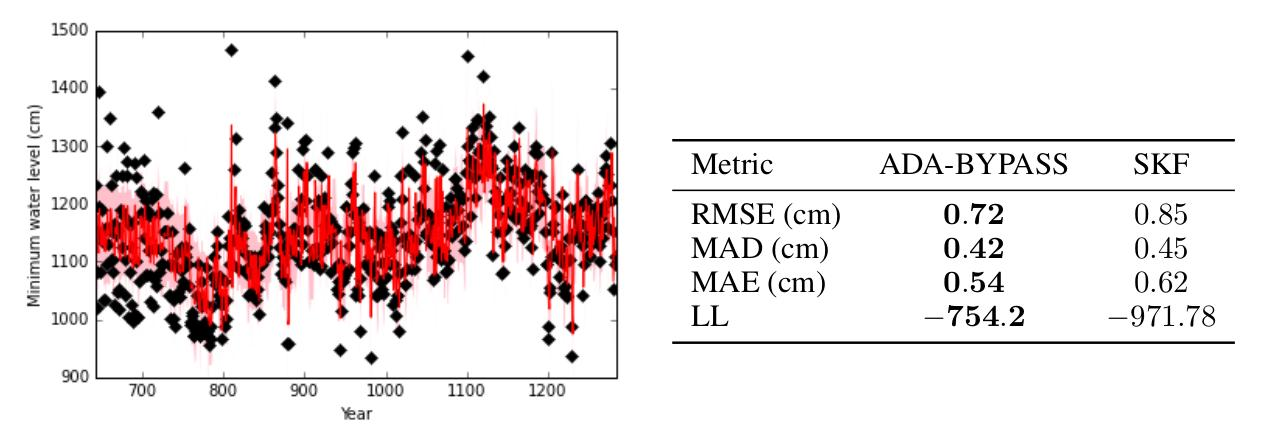
\includegraphics[width=\textwidth, keepaspectratio]{nile}
\caption{Online one-year ahead predictions for the Nile’s minimum water levels. Left panel: observed levels (black diamonds), predicted levels (red line) and ±1 standard deviation error bars
(pink area). Right panel: predictive performances; error metrics shown are root mean squared error (RMSE), mean absolute deviation (MAD), mean absolute error (MAE) and predictive log likelihood
(LL).}
\label{fig:nile}
\end{figure}

\subsubsection{Wind speed data}

To demonstrate the superior performance of ADA-BYPASS on a large data set, we next present the series of anemometer wind speed measurements (in m/s) from a Danish wind turbine. The data were sampled at ten-minute intervals for just over nine months, resulting in a total of 40,174 measurements. The ten-minute lookahead predictive performance achieved by each method is reported in Table~\ref{tab:windspeed}.
\begin{table}[t]
\caption{Predictive performance of ADA-BYPASS vs SKF on the wind speed data set.}
\label{tab:windspeed}
\centering
  \begin{tabular}{lcc}
    \toprule
    Metric    & ADA-BYPASS     & SKF \\
    \midrule
    RMSE (m/s) & \textbf{0.6}  & 0.64     \\
    MAD (m/s)     & \textbf{0.3} & 0.31      \\
    MAE (m/s)     & \textbf{0.42}       & 0.44  \\
    LL     & \textbf{-24,971.75}       & -30,140.04  \\
    \bottomrule
  \end{tabular}
\end{table}

\subsubsection{Statistical arbitrage}

LGSSMs, and variants thereof, have seen a widespread use in statistical arbitrage strategies, notably in pairs trading \citep{epchan, triantafyllopoulos11, montana09}. In this area, they serve as a dynamic model for the price spread between two assets. In our application, we seek to find the \emph{hedge ratio}\footnote{The hedge ratio of a particular asset is the number of units of that asset we should buy or sell in a portfolio. If the asset is a stock, then the number of units corresponds to the number of shares. A negative hedge ratio indicates we should sell that asset.} and the predictive standard deviation of the spread. The observable variable is thus one of the price series $y$, and the hidden variable is the hedge ratio $w$. We assume that both variables can be modelled via the following measurement and transition equations, respectively:
\begin{align}
	& y_t = w_t x_t + u_t, \qquad u_t \sim \mathcal{N}(u_t | \mu, \beta^{-1}),
	\\
	& w_t = w_{t-1} + \xi_t, \qquad \xi_t \sim \mathcal{N}(\xi_t | 0, \alpha^{-1}),
\end{align}
where $x$ is the price series of the other asset. Typically, $\alpha$, $\beta$ and $\mu$ are manually selected in hindsight \citep{epchan}. However, this practice is highly prone to the so-called \emph{data-snooping bias}: these parameters can be tweaked so as to optimise the backtesting performance of the strategy. The ADA-BYPASS algorithm automatically tunes its underlying parameters, so it does not suffer from this caveat.

We tested ADA-BYPASS on a pair of exchange-traded funds (ETFs) consisting of the SPDR gold trust GLD and the gold-miners ETF GDX. This ETF pairing is a favourite in the financial industry, because the value of gold-mining companies is very much based on the value of gold. We downloaded the corresponding, daily adjusted closing prices from Yahoo! Finance, between May 22, 2006 and April 22, 2015.

Rather than maximising profits, most investors attempt to maximise risk-adjusted returns, as advocated by modern portfolio theory. The Sharpe ratio is the most widely used measure of risk-adjusted returns \citep{sharpe}. Besides the Sharpe ratio, the maximum drawdown and maximum drawdown duration are two other popular metrics to evaluate trading strategies. From Table~\ref{tab:statarb}, we can clearly discern that ADA-BYPASS beats SKF by a significant margin in terms of the aforementioned performance metrics.
%\begin{table}[t]
%\caption{Performance of the GDX-GLD pairs trade under ADA-BYPASS and SKF.}
%\label{tab:statarb}
%\centering
%  \begin{tabular}{lcc}
%    \toprule
%    Metric    & ADA-BYPASS     & SKF \\
%    \midrule
%    Sharpe ratio & \textbf{1.12}  & 0.7     \\
%    Maximum drawdown (\%)     & \textbf{14.61} & 73.05      \\
%    Maximum drawdown duration (trading days)     & \textbf{375}       & 567  \\
%    \bottomrule
%  \end{tabular}
%\end{table}
\begin{table}[t]
\caption{Performance of the GDX-GLD pairs trade under ADA-BYPASS and SKF.}
\label{tab:statarb}
\centering
  \begin{tabular}{lcc}
    \toprule
    Metric    & ADA-BYPASS     & SKF \\
    \midrule
    Sharpe ratio & \textbf{1.00}  & 0.70     \\
    Maximum drawdown (\%)     & \textbf{15.93} & 73.05      \\
    Maximum drawdown duration (trading days)     & \textbf{404}       & 567  \\
    \bottomrule
  \end{tabular}
\end{table}

\begin{mccorrection}
\subsection{Impact of different priors}
\end{mccorrection}

In order to gauge the effects of our proposed Bayesian approach, we shall in this section check the impact of different means and standard deviations of the prior weight distributions\footnote{We shall not, however, analyse the impact of different classes of prior distributions, as that would move us too far away from the PA regression context which, as we saw from Eqs. \eqref{eq:PA-I-optpb-altform} and \eqref{eq:PA-I-optpb}, implicitly imposes a Gaussian prior over its weights.}. Since the entire focus and pillar of this thesis are financial applications, we shall just rerun the statistical arbitrage experiment from the previous section under different means for the weight prior, but keeping the variance constant at 0. The relevant metrics are presented in Table~\ref{tab:statarb2}.
\begin{table}[H]
\caption{Performance of the GDX-GLD pairs trade under ADA-BYPASS, with different prior means $\mu$ (picked arbitrarily) and constant, zero variance.}
\label{tab:statarb2}
\centering
\scalebox{0.75}{
  \begin{tabular}{lccccccc}
    \toprule
    Metric    & $\mu=-10$ & $\mu=-2$ & $\mu=-1$ & $\mu=0$ & $\mu=1$ & $\mu=2$ & $\mu=10$ \\
    \midrule
    Sharpe ratio & 1.01 & 0.98 & 0.91 & 1.00 & 0.94 & 1.06 & 1.01 \\
    Maximum drawdown (\%)     & 14.72 & 15.51 & 15.69 & 15.93 & 16.55 & 16.00 & 13.74    \\
    Maximum drawdown duration (trading days)     & 379 & 628     & 536 & 404 & 342 & 359 & 319  \\
    \bottomrule
  \end{tabular}
}
\end{table}
The table shows that, within reason, the performance of the model is not critical upon the values of the weight prior mean ($\mu$) tested. That is as we may have expected.



\section{Concluding Remarks}

In this chapter, we stated the shortcomings of online passive-aggressive (PA) algorithms and discussed ways to overcome them. In particular, we introduced generalised passive-aggressive learning which enables the use of \emph{any} loss function within the PA framework (which, as a reminder, is restricted to the hinge loss for classification and the $\epsilon$-insensitive loss for regression).

We also developed the first online Bayesian PA regression model within the state-space setting, along with a novel, online variational inference algorithm. This model is ideal for the probabilistic prediction of non-stationary and/or very large time series, in particular massive, time-varying data streams. Results on three real-world data sets show significant improvements in predictive performance over a more standard LGSSM.

\begin{mccorrection}
One of the criticisms that could be directed at our work in this section is the absence of any evidence for why our proposed online hyperparameter tuning mechanism provides benefits, if any, over the most straightforward approach one could think of, i.e. cross-validation (CV). Although it would be possible to perform cross-validation with a rolling or sliding window, one of fundamental ideologies behind the thesis was to have online algorithms for portfolio management with the \textbf{fewest} to-be-manually-tuned hyperparameters as possible (so as to avoid data-snooping bias). Going down the rolling-window CV path goes against this fundamental ideology, as it introduces another layer of hyperparameters to be manually chosen by the practitioner (in addition to those she is trying to tune in the first place), namely 1) the size of the rolling window, 2) the size of the CV leave-out sets and 3) the CV frequency (i.e., how often do you perform CV?). For these reasons, we shall not consider rolling CV in this thesis altogether.
\end{mccorrection}